\documentclass[dvipsnames]{beamer}
\usepackage[utf8]{inputenc}
\usepackage{listings}
\usepackage{comment}
\usepackage{soul}
%\usepackage{ulem}
\usepackage{subfig}
\setul{}{1pt}
\usepackage[oldenum, olditem]{paralist}
%allow even smaller text
\newcommand\tinytiny{\fontsize{4pt}{3}\selectfont}

\makeatletter
\let\old@lstKV@SwitchCases\lstKV@SwitchCases
\def\lstKV@SwitchCases#1#2#3{}
\makeatother
\usepackage{lstlinebgrd}
\makeatletter
\let\lstKV@SwitchCases\old@lstKV@SwitchCases

\lst@Key{numbers}{none}{%
    \def\lst@PlaceNumber{\lst@linebgrd}%
    \lstKV@SwitchCases{#1}%
    {none:\\%
     left:\def\lst@PlaceNumber{\llap{\normalfont
                \lst@numberstyle{\thelstnumber}\kern\lst@numbersep}\lst@linebgrd}\\%
     right:\def\lst@PlaceNumber{\rlap{\normalfont
                \kern\linewidth \kern\lst@numbersep
                \lst@numberstyle{\thelstnumber}}\lst@linebgrd}%
    }{\PackageError{Listings}{Numbers #1 unknown}\@ehc}}
\makeatother


\graphicspath{{logos/}}

%disclaimer for Sandia. uncomment and the whole blob goes away @ b80c116300122
\def\sandid{SAND2020-8508 PE}

% \title{Performance Portability with Kokkos}
\title{The Kokkos Lectures}

%BAD misuse of author field
\author{Module 5: SIMD, Streams and Tasking}

%\author{
%  Jeff Miles \inst{1},
%  Christian Trott \inst{1}
%}
%\institute[shortinst]{\tiny \inst{1} Sandia National Laboratories, \inst{2} Oak Ridge National Laboratory \and \inst{3} Los Alamos National Laboratory}
%\institute[shortinst]{\tiny \inst{1} Sandia National Laboratories}

\usetheme{kokkos}

\newif\ifshort
\newif\ifmedium
\newif\iffull
\newif\ifnotoverview

\newcommand{\TutorialDirectory}{\texttt{Intro-Full}}
\newcommand{\ExerciseDirectory}[1]{\texttt{Exercises/#1/}}
\newcommand{\TutorialClone}{\texttt{Kokkos/kokkos-tutorials/\TutorialDirectory}}

\definecolor{darkgreen}{rgb}{0.0, 0.5, 0.0}
\definecolor{darkred}{rgb}{0.8, 0.0, 0.0}
\definecolor{orange}{rgb}{0.8, 0.33, 0.0}
\definecolor{purple}{rgb}{0.60, 0.20, 0.80}
\colorlet{bodyColor}{blue!20}
\colorlet{patternColor}{orange!30}
\colorlet{policyColor}{green!30}

% http://tex.stackexchange.com/questions/144448/color-a-text-line-in-a-code-lstlisting
\lstnewenvironment{code}[1][]%
{
  %with txfonts: OT1/txr/m/n/10
  %with default fonts: OT1/cmr/m/n/10
  %\fontfamily{cmr}\selectfont
  %\showthe\font
   \noindent
   \minipage{\linewidth}
   %\vspace{0.5\baselineskip}
   \lstset{mathescape, escapeinside={<@}{@>},
moredelim=**[is][{\btHL[fill=patternColor]}]{@pattern}{@pattern},
moredelim=**[is][{\btHL[fill=red!30]}]{@warning}{@warning},
moredelim=**[is][{\btHL[fill=policyColor]}]{@policy}{@policy},
moredelim=**[is][{\btHL[fill=bodyColor]}]{@body}{@body},
moredelim=**[is][{\btHL[fill=red!30]}]{@warning}{@warning},
moredelim=**[is][\color{black}]{@black}{@black},
moredelim=**[is][\color{blue}]{@blue}{@blue},
moredelim=**[is][\bf]{@bold}{@bold},
moredelim=**[is][\it]{@italic}{@italic},
moredelim=**[is][\color{boldblue}\bf]{@boldblue}{@boldblue},
moredelim=**[is][\color{red}]{@red}{@red},
moredelim=**[is][\color{green}]{@green}{@green},
moredelim=**[is][\color{gray}]{@gray}{@gray},
moredelim=**[is][\color{darkgreen}]{@darkgreen}{@darkgreen},
moredelim=**[is][\color{darkred}]{@darkred}{@darkred},
moredelim=**[is][\color{orange}]{@orange}{@orange},
moredelim=**[is][\color{purple}]{@purple}{@purple},
keywords={},
#1}
}
{
  \endminipage
  %\vspace{1.0\baselineskip}
}

\makeatletter
\newif\ifATOlinebackground
\lst@Key{linebackground}{\tiny}{\def\ATOlinebackground{#1}\global\ATOlinebackgroundtrue}
\makeatother

\lstnewenvironment{shell}[1][]{%
  \global\ATOlinebackgroundfalse
  \lstset{language=sh,%
    showstringspaces=false,
    aboveskip=0pt,
    frame=none,
    numbers=none,
    belowskip=2pt,
    breaklines=true,
    #1,
    }
  %\ifATOlinebackground
  \lstset{linebackgroundcolor={
    \ATOlinebackground
  }}
  %\fi
  }{}

\lstnewenvironment{cmake}[1][]{%
  \global\ATOlinebackgroundfalse
  \lstset{language=sh,%
    showstringspaces=false,
    aboveskip=0pt,
    frame=none,
    numbers=none,
    belowskip=2pt,
    breaklines=true,
    #1,
    }
  %\ifATOlinebackground
  \lstset{linebackgroundcolor={
    \ATOlinebackground
  }}
  %\fi
  }{}

\newcommand{\inlinecode}[1]{{\lstset{basicstyle=\ttfamily,keywordstyle={},showstringspaces=false}\lstinline$#1$}}
\newcommand{\inlineshell}[1]{{\lstset{basicstyle=\ttfamily,keywordstyle={},showstringspaces=false}\lstinline$#1$}}

\setbeamercolor{block title}{fg=white, bg=SandiaLightBlue}
\setbeamercolor{block body}{bg=lightgray}
\setbeamercolor{block title alerted}{fg=white, bg=SandiaRed}
\setbeamercolor{block body alerted}{bg=lightgray}



%\usepackage[texcoord,grid,gridunit=mm,gridcolor=red!10,subgridcolor=green!10]{eso-pic}
\usepackage[absolute,overlay]{textpos}





% http://tex.stackexchange.com/questions/8851/how-can-i-highlight-some-lines-from-source-code

\usepackage{pgf, pgffor}
\usepackage{listings}
\usepackage{lstlinebgrd} % see http://www.ctan.org/pkg/lstaddons

\makeatletter
%%%%%%%%%%%%%%%%%%%%%%%%%%%%%%%%%%%%%%%%%%%%%%%%%%%%%%%%%%%%%%%%%%%%%%%%%%%%%%
%
% \btIfInRange{number}{range list}{TRUE}{FALSE}
%
% Test in int number <number> is element of a (comma separated) list of ranges
% (such as: {1,3-5,7,10-12,14}) and processes <TRUE> or <FALSE> respectively

\newcount\bt@rangea
\newcount\bt@rangeb

\newcommand\btIfInRange[2]{%
    \global\let\bt@inrange\@secondoftwo%
    \edef\bt@rangelist{#2}%
    \foreach \range in \bt@rangelist {%
        \afterassignment\bt@getrangeb%
        \bt@rangea=0\range\relax%
        \pgfmathtruncatemacro\result{ ( #1 >= \bt@rangea) && (#1 <= \bt@rangeb) }%
        \ifnum\result=1\relax%
            \breakforeach%
            \global\let\bt@inrange\@firstoftwo%
        \fi%
    }%
    \bt@inrange%
}
\newcommand\bt@getrangeb{%
    \@ifnextchar\relax%
        {\bt@rangeb=\bt@rangea}%
        {\@getrangeb}%
}
\def\@getrangeb-#1\relax{%
    \ifx\relax#1\relax%
        \bt@rangeb=100000%   \maxdimen is too large for pgfmath
    \else%
        \bt@rangeb=#1\relax%
    \fi%
}

%%%%%%%%%%%%%%%%%%%%%%%%%%%%%%%%%%%%%%%%%%%%%%%%%%%%%%%%%%%%%%%%%%%%%%%%%%%%%%
%
% \btLstHL<overlay spec>{range list}
%
% TODO BUG: \btLstHL commands can not yet be accumulated if more than one overlay spec match.
%
\newcommand<>{\btLstHL}[2]{%
  \only#3{\btIfInRange{\value{lstnumber}}{#1}{\color{#2}\def\lst@linebgrdcmd{\color@block}}{\def\lst@linebgrdcmd####1####2####3{}}}%
}%
\makeatother






% http://tex.stackexchange.com/questions/15237/highlight-text-in-code-listing-while-also-keeping-syntax-highlighting
%\usepackage[T1]{fontenc}
%\usepackage{listings,xcolor,beramono}
\usepackage{tikz}

\makeatletter
\newenvironment{btHighlight}[1][]
{\begingroup\tikzset{bt@Highlight@par/.style={#1}}\begin{lrbox}{\@tempboxa}}
{\end{lrbox}\bt@HL@box[bt@Highlight@par]{\@tempboxa}\endgroup}

\newcommand\btHL[1][]{%
  \begin{btHighlight}[#1]\bgroup\aftergroup\bt@HL@endenv%
}
\def\bt@HL@endenv{%
  \end{btHighlight}%
  \egroup
}
\newcommand{\bt@HL@box}[2][]{%
  \tikz[#1]{%
    \pgfpathrectangle{\pgfpoint{1pt}{0pt}}{\pgfpoint{\wd #2}{\ht #2}}%
    \pgfusepath{use as bounding box}%
    \node[anchor=base west, fill=orange!30,outer sep=0pt,inner xsep=1pt, inner ysep=0pt, rounded corners=3pt, minimum height=\ht\strutbox+1pt,#1]{\raisebox{1pt}{\strut}\strut\usebox{#2}};
  }%
}
\makeatother



\usetikzlibrary{calc}
\usepackage{xparse}%  For \NewDocumentCommand

% tikzmark command, for shading over items
\newcommand{\tikzmark}[1]{\tikz[overlay,remember picture] \node (#1) {};}

\makeatletter
\NewDocumentCommand{\DrawBox}{s O{}}{%
    \tikz[overlay,remember picture]{
    \IfBooleanTF{#1}{%
        \coordinate (RightPoint) at ($(left |- right)+(\linewidth-\labelsep-\labelwidth,0.0)$);
    }{%
        \coordinate (RightPoint) at (right.east);
    }%
    \draw[red,#2]
      ($(left)+(-0.2em,0.9em)$) rectangle
      ($(RightPoint)+(0.2em,-0.3em)$);}
}

\NewDocumentCommand{\DrawBoxWide}{s O{}}{%
    \tikz[overlay,remember picture]{
    \IfBooleanTF{#1}{%
        \coordinate (RightPoint) at ($(left |- right)+(\linewidth-\labelsep-\labelwidth,0.0)$);
    }{%
        \coordinate (RightPoint) at (right.east);
    }%
    \draw[red,#2]
      ($(left)+(-\labelwidth,0.9em)$) rectangle
      ($(RightPoint)+(0.2em,-0.3em)$);}
}

\NewDocumentCommand{\DrawBoxWideBlack}{s O{}}{%
    \tikz[overlay,remember picture]{
    \IfBooleanTF{#1}{%
        \coordinate (RightPoint) at ($(left |- right)+(\linewidth-\labelsep-\labelwidth,0.0)$);
    }{%
        \coordinate (RightPoint) at (right.east);
    }%
    \draw[black,#2]
      ($(left)+(-\labelwidth,0.9em)$) rectangle
      ($(RightPoint)+(0.2em,-0.3em)$);}
}
\makeatother

\usetikzlibrary{positioning}

\usetikzlibrary{shapes}

\hypersetup{
    colorlinks=true,
    linkcolor=blue,
    filecolor=magenta,
    urlcolor=cyan,
}



\shortfalse
\mediumtrue
\fulltrue
\notoverviewtrue

\begin{document}

% \begin{frame}
%   \titlepage
% \end{frame}
% 
%==============================================================================

\begin{frame}{NVIDIA's NVLABS LOGISTICS (1)}

\textbf{\large SOFTWARE FOR LAB}

\vspace{10pt}

\textbf{Remote Desktop Software:} \\
\begin{itemize}
\item {Download NoMachine now for best performance from \\
 \textbf{\ul{www.nomachine.com/download}}}
\item {Alternatively you may use a VNC client or the provided browser-based VNC option}
\end{itemize}

\vspace{10pt}

\textbf{SSH Access Software (optional):}
\begin{itemize}
\item PuTTy for Windows can be downloaded from \textbf{\ul{www.putty.org}}
\item{Alternatively you may use a provided browser-based SSH option}
\end{itemize}

\end{frame}

%==============================================================================

\begin{frame}{NVIDIA's NVLABS LOGISTICS (2)}

\textbf{\Large CONNECTION INSTRUCTIONS}
\begin{itemize}
\item {Navigate to \textbf{\ul{nvlabs.qwiklab.com}}}
\item {Login or create a new account}
\item {Select the \textbf{Instructor-Led Hands-on Labs} Class}
\item {Find the lab called \textbf{Kokkos, ...}, select it, click Select, and finally click Start}
\item {After a short wait, lab instance Connection information will be shown}
\item {Please ask Lab Assistants for help!}
\end{itemize}

\end{frame}

%==============================================================================



\begin{frame}
	\titlepage
\end{frame}

\begin{frame}{Welcome to Kokkos}

\textbf{Online Resources}:

\begin{itemize}
        \item \url{https://github.com/kokkos}:
                \begin{itemize}
                        \item Primary Kokkos GitHub Organization
                \end{itemize}
        \item \url{https://kokkos.org/kokkos-core-wiki/videolectures.html}
                \begin{itemize}
			\item{Slides, recording and Q\&A for the lectures}
                \end{itemize}
        \item \url{https://kokkos.org/kokkos-core-wiki}:
                \begin{itemize}
                        \item Programming guide and API reference documentation
                \end{itemize}
        \item \url{https://kokkosteam.slack.com}:
                \begin{itemize}
                        \item Slack channel for Kokkos.
                        \item Please join: fastest way to get your questions answered.
                        \item Can whitelist domains, or invite individual people.
                \end{itemize}
\end{itemize}

\end{frame}


\begin{frame}[fragile]{Lecture Series Outline}

\begin{itemize}
        \item Module 1: Introduction, Building and Parallel Dispatch
        \item Module 2: Views and Spaces
        \item Module 3: Data Structures + MultiDimensional Loops
        \item Module 4: Hierarchical Parallelism
        \item \textbf{Module 5: SIMD, Streams and Tasking}
        \item Module 6: Internode: MPI and PGAS
        \item Module 7: Tools: Profiling, Tuning and Debugging
        \item Module 8: Kernels: Sparse and Dense Linear Algebra
        \item Module 9: Fortran inter-op
\end{itemize}

\end{frame}



\begin{frame}[fragile]{Module 4: Summary}
	\textbf{Hierarchal Parallelism}
  \begin{itemize}
    \item{\textbf{Hierarchical work} can be parallelized via hierarchical parallelism.}
    \item{Hierarchical parallelism is leveraged using \textbf{thread teams} launched with a \texttt{TeamPolicy}.}
    \item{Team ``worksets'' are processed by a team in nested \texttt{parallel\_for} (or \texttt{reduce} or \texttt{scan}) calls with a \texttt{TeamThreadRange} and \texttt{ThreadVectorRange} policy.}
    \item{Execution can be restricted to a subset of the team with the \texttt{single} pattern using either a \texttt{PerTeam} or \texttt{PerThread} policy.}
    \item{Teams can be used to \textbf{reduce contention} for global resources even in ``flat'' algorithms.}
  \end{itemize}


  
\end{frame}

\begin{frame}[fragile]{Module 4: Summary}
   \textbf{Scratch Space}
\begin{itemize}
    \item{\textbf{Scratch Memory} can be use with the \texttt{TeamPolicy} to provide thread or team \textbf{private} memory.}
    \item{Usecase: per work-item temporary storage or manual caching.}
    \item{Scratch memory exposes on-chip user managed caches (e.g. on NVIDIA GPUs)}
    \item{The size must be determined before launching a kernel.}
    \item{Two levels are available: large/slow and small/fast.}
  \end{itemize}
  \textbf{Unique Token}
  \begin{itemize}
    \item{\textbf{UniqueToken} give a thread safe portable way to divide thread specific resources}
    \item{\textbf{UniqueToken} can be sized to restrict ids to a range.}
    \item{A \textbf{Global} UniqueToken is available.}
  \end{itemize}

\end{frame}

\begin{frame}{Module 5}
  \begin{block}{SIMD}
    How to vectorize code with explicit vector types.
  \end{block}

  \begin{block}{Blocking behavior and Execution Space Instances}
    What is Kokkos's blocking behavior and Execution Space Instances
  \end{block}

  \begin{block}{Tasking}
    Writing dynamic task graphs.
  \end{block}
\end{frame}


%==========================================================================

\begin{frame}[fragile]

  {\Huge SIMD}

  \vspace{10pt}

  {\large Portable vector intrinsic types.}

  \vspace{20pt}

  \textbf{Learning objectives:}
  \begin{itemize}
    \item {How to use SIMD types to improve vectorization.}
    \item {SIMD Types as an alternative to ThreadVector loops.}
    \item {SIMD Types to achieve outer loop vectorization.}
  \end{itemize}

  \vspace{-20pt}

\end{frame}

%==========================================================================

\begin{frame}[fragile]{Vectorization In Kokkos}

   So far there were two options for achieving vectorization: 

\begin{itemize}
  \item{{\textbf{Hope For The Best}}: Kokkos semantics make loops inherently vectorizable, sometimes the compiler figures it even out.}
  \item{{\textbf{Hierarchical Parallelism}}: {\texttt{TeamVectorRange}} and {\texttt{ThreadVectorRange}} help the compiler with hints such as {\texttt{\#pragma ivdep}} or {\texttt{\#pragma omp simd}}}.
\end{itemize}

   \vspace{3pt}

  These strategies do run into limits though:

\begin{itemize}
  \item{Compilers often do not vectorize loops on their own.}
  \item{An optimal vectorization strategy would require \emph{outer-loop vectorization}.}
  \item{Vectorization with \texttt{TeamVectorRange} sometimes requires artifically introducing an additional loop level.}
\end{itemize}
\end{frame}

\begin{frame}[fragile]{Outer-Loop Vectorization}

   A simple scenario where for outer-loop vectorization:
	\vspace{-3pt}
  \begin{code}[linebackgroundcolor={},keywords={for,int}]
  for(int i=0; i<N; i++) {
    // expect K to be small odd 1,3,5,7 for physics reasons
    for(int k=0; k<K; k++) b(i) += a(i,k);
  }
  \end{code}

  Vectorization the \texttt{K}-Loop is not profitable:
  \begin{itemize}
	  \item{It is a short reduction.}
	  \item{Remainders will eat up much time.}
  \end{itemize}
	\vspace{5pt}

  Using \texttt{ThreadVectorRange} is cumbersome and requires split of \texttt{N}-Loop:

  \begin{code}[linebackgroundcolor={},keywords={parallel_for,for,int,TeamPolicy,ThreadVectorRange}]
parallel_for("VectorLoop",TeamPolicy<>(0,N/V,V),
  KOKKOS_LAMBDA ( const team_t& team ) {
  int i = team.league_rank() * V;
  for(int k=0; k<K; k++) 
    parallel_for(ThreadVectorRange(team,V), [&](int ii) {
      b(i+ii) += a(i+ii,k);
    });
});
    \end{code}
\end{frame}

\begin{frame}[fragile]{SIMD Types}
  
   To help with this situation and (in particular in the past) fix the lack of auto-vectorizing compilers \texttt{SIMD-Types} have been invented. They:
	\begin{itemize}
		\item{Are short vectors of scalars.}
		\item{Have operators such as \texttt{+=} so one can use them like scalars.}
		\item{Are compile time sized.}
		\item{Usually map directly to hardware vector instructions.}
	\end{itemize}
	
	\begin{block}{Important concept: SIMD Type}
		A SIMD variable is a \textbf{short vector} which acts like a scalar.
  \end{block}

	Using such a \texttt{simd} type one can simply achieve \emph{outer-loop} vectorization by using arrays of \texttt{simd} and dividing the loop range by its \emph{size}.
\end{frame}

\begin{frame}[fragile]{Outer-Loop Vectorization}

  Lets take a look back at the outer loop vectorization:
  \begin{code}[linebackgroundcolor={},keywords={for,int}]
  View<double*> b = ...
  View<double**> a = ...
  for(int i=0; i<N; i++) {
    // expect K to be small odd 1,3,5,7 for physics reasons
    for(int k=0; k<K; k++) b(i) += a(i,k);
  }
  \end{code}

  \pause
  Using SIMD types is conceptionally as simple as:
	\begin{itemize}
		\item Replace scalar type with SIMD type
		\item Adjust loop iteration count by SIMD length
	\end{itemize}

  \begin{code}[linebackgroundcolor={},keywords={for,int}]
  using simd_t = Kokkos::Experimental::simd<double, Kokkos::Experimental::simd_abi::native>;
  View<simd_t*> b = ...
  View<simd_t**> a = ...
  int V = simd_t::size();
  for(int i=0; i<N/V; i++) {
    // expect K to be small odd 1,3,5,7 for physics reasons
    for(int k=0; k<K; k++) b(i) += a(i,k);
  }
  \end{code}
\end{frame}

\begin{frame}[fragile]{C++23? SIMD}
	The ISO C++ standard has a \emph{Technical Specification} for \texttt{simd} (in \emph{parallelism v2}):

  \begin{code}[linebackgroundcolor={},keywords={template,class,public,using}]
template< class T, class Abi >
class simd {
public:
  using value_type = T;
  using reference = /* impl defined */;
  using abi_type = Abi;
  static constexpr size_t size();
  void copy_from(T const*, aligned_tag);
  void copy_to(T*, aligned_tag) const;
  T& operator[] (size_t);
  //Element wise operators
};

// Element Wise non-member operators

  \end{code}

\end{frame}

\begin{frame}[fragile]{C++23? SIMD ABI}
One interesting innovation here is the \texttt{Abi} parameter allowing for different, hardware specific, implementations.

	\vspace{8pt}

The most important in the proposal are:
\begin{itemize}
	\item{\textbf{scalar}: single element type.}
	\item{\textbf{native}: best fit for hardware.}
        \item{\textbf{fixed\_size$<$N$>$}: stores N elements. NOT YET IN KOKKOS.}
\end{itemize}

\pause
	\vspace{8pt}

	But \texttt{std::simd} is not in the standard yet, and doesn't support GPUs ...

	\pause
	\vspace{8pt}
	It also has other problems making it insufficient for our codes ...
\end{frame}

\begin{frame}[fragile]{Kokkos SIMD}
   Just at Sandia we had at least \textbf{5} different SIMD types in use.

   \vspace{8pt}
   A unification effort was started with the goal of:
   \begin{itemize}
      \item{Match the proposed \texttt{std::simd} API as far as possible.}
      \item{Support GPUs.}
      \item{Can be used stand-alone or in conjunction with Kokkos.}
      \item{Replaces all current implementations at Sandia for SIMD.}
   \end{itemize}

\end{frame}

\begin{frame}[fragile]{Kokkos SIMD}
  As with the C++23 SIMD type it takes Scalar argument and ABI
  \begin{code}
     template<class Scalar, class ABI>
     simd;
  \end{code}

  Two supported ABIs are:
  \begin{itemize}
     \item \texttt{simd\_abi::native}: whatever is best for the scalar type on the architecture
     \item \texttt{simd\_abi::scalar}: a single element
  \end{itemize}

  Aliasing with Scalar Views is possible (but careful with Layout and length!)
  \begin{code}
using simd_t = simd<double, simd::simd_abi::native>;
View<simd_t*> a("A",N);
View<double*> a_s(static_cast<double*>(a.data()),N*simd_t::size());
     
View<double*> b("B",M);
View<simd_t*> b_v(static_cast<simd_t*>(b.data()),M/simd_t::size());
  \end{code}

\end{frame}

\begin{frame}[fragile]{Exercise: Simple SIMD usage.}

  \textbf{Details}:
  \begin{small}
  \begin{itemize}
\item Location: \ExerciseDirectory{simd/Begin}
\item Include the \texttt{simd.hpp} header.
\item Change the data type of the views to use \texttt{simd$<$double, simd\_abi:native$>$}.
\item Create an unmanaged \texttt{View$<$double*$>$} of \texttt{results} using the \texttt{data()} function for the final reduction.  
\end{itemize}
  \end{small}

\begin{code}
   # Compile for CPU
   make -j KOKKOS_DEVICES=OpenMP
   # Compile for GPU
   make -j KOKKOS_DEVICES=Cuda
   # Run on GPU
   ./simd.cuda
\end{code}

	\vspace{-3pt}
\ul{\textbf{Things to try:}}
  \begin{small}
  \begin{itemize}
  \item Vary problem size (-N ...; -K ...)
  \item Compare behavior of scalar vs vectorized on CPU and GPU
  \end{itemize}
  \end{small}



\end{frame}

\begin{comment}
\begin{frame}[fragile]{The GPU SIMD Problem}
  The above exercise used a \textbf{scalar} simd type on the \textbf{GPU}.
  
	{\textbf Why wouldn't we use a fixed\_size instead?}

	\begin{itemize}
	   \item{Using a \texttt{fixed\_size} ABI will create a scalar of size \texttt{N} in each CUDA thread!}
	   \item{Loading a \texttt{fixed\_size} variable from memory would result in uncoalesced access.}
           \item{If you have correct layouts you get \texttt{outer-loop} vectorization implicitly on GPUs.}
	\end{itemize}

	\pause
	But what if you really want to use \textbf{warp}-level parallelization for SIMD types?

	\pause
	{\textbf We need \emph{two} SIMD types: a \emph{storage} type and a \emph{temporary} type!}
\end{frame}

\begin{frame}[fragile]{cuda\_warp ABI}
  \begin{block}{Important concept: simd::storage\_type}
    Every \texttt{simd$<$T,ABI$>$} has an associated \texttt{storage\_type} typedef.
  \end{block}

  To help with the GPU issue we split types between \textbf{storage} types used for \texttt{Views}, and \textbf{temporary} variables.

  \begin{itemize}
	  \item{Most \texttt{simd::simd} types will just have the same \texttt{storage\_type}.}
	  \item{\texttt{simd$<$T,cuda\_warp$<$N$> >$} will use warp level parallelism.}
	  \item{\texttt{simd$<$T,cuda\_warp$<$N$> >$::storage\_type} is different though!}
	  \item{Used in conjunction with \texttt{TeamPolicy}.}
  \end{itemize}
\end{frame}

\begin{frame}[fragile]{cuda\_warp ABI}
\textbf{Illustrating difference between \texttt{pack} and \texttt{cuda\_warp}}


      \begin{code}[linebackgroundcolor={},keywords={simd,parallel_for,using}]
using ABI = ... ;
View<simd<double,ABI::storage_type> A(...);
parallel_for(TeamPolicy<>(N,AUTO,V), 
 KOKKOS_LAMBDA(const teamt_t& team) {
  int i = team.league_rank()*team.team_size()+team.team_rank();
  simd<double,ABI> tmp = A(i);
});
       \end{code}
  \begin{columns}[]
    \begin{column}{.5\textwidth}
      \begin{code}[linebackgroundcolor={},keywords={pack,using}]
using ABI = pack<8>; int V=1;
\end{code}

       \includegraphics[width=0.75\textwidth]{figures/simd-fixedsize} 

    \end{column}
    \begin{column}{.5\textwidth}
      \begin{code}[linebackgroundcolor={},keywords={cuda_warp,using}]
using ABI = cuda_warp<8>; int V=8;
\end{code}

       \includegraphics[width=0.75\textwidth]{figures/simd-warp} 

    \end{column}
  \end{columns}
\end{frame}

\begin{frame}[fragile]{cuda\_warp ABI}

Example of using \texttt{storage\_type}:

\begin{code}[linebackgroundcolor={},keywords={template,class,simd,simd_storage,TeamPolicy,TeamThreadRange,public,using}]
// Using cuda_warp abi
using simd_t = simd::simd<T,simd::simd_abi::cuda_warp<V> >;
// Define simd_storage type
using simd_storage_t = simd_t::storage_type;
// Allocate memory
View<simd_storage_t**> data("D",N,M); // will hold N*M*V Ts

// Launch Loop with vectorlength V
parallel_for("Loop", TeamPolicy<>(N,M,V), 
  KOKKOS_LAMBDA(const team_t& team) {
    int i = team.league_rank();
    parallel_for(TeamThreadRange(team,M), [&](int j) {
      // Load storage type into internal type;
      simd_t tmp = data(i,j);
      // Do something with it
      tmp *= 2.0;
      // write values back
      data(i,j) = tmp;
      // or inline:
      // data(i,j) = 2.0*simd_t(data(i,j));
  }); 
});
\end{code}

\end{frame}


\begin{frame}[fragile]{Exercise: SIMD storage usage.}

  \textbf{Details}:
  \begin{small}
  \begin{itemize}
\item Location: \ExerciseDirectory{simd\_warp/Begin}
\item Include the \texttt{simd.hpp} header.
\item Change the data type of the views to use \texttt{simd::simd$<$double,simd::simd\_abi:cuda\_warp$<32>>$::storage\_type}.
\item Create an unmanaged \texttt{View$<$double*$>$} of \texttt{results} using the \texttt{data()} function for the final reduction.  
\item Use inside of the lambda the \texttt{simd::simd$<$double,simd::simd\_abi:cuda\_warp$<32>>$} as scalar type.
\end{itemize}
  \end{small}

\begin{code}
   # Compile for GPU
   make -j KOKKOS_DEVICES=Cuda
   # Run on GPU
   ./simd.cuda
\end{code}

\end{frame}
\end{comment}

\begin{frame}[fragile]{Advanced SIMD Capabilities}

Kokkos SIMD supports math operations:
\begin{itemize}
  \item{Common stuff like \texttt{abs}, \texttt{sqrt}, \texttt{exp}, ...}
\end{itemize}

\vspace{8pt}
It also supports masking:

	\begin{code}
// Scalar code with condition:
for(int i=0; i<N; i++) {
  if( a(i) < 100.0 ) b(i) = a(i);
  else b(i) = 100.0;
}

// Becomes
using simd_t = simd<double,simd_abi::native>;
using simd_mask_t = simd_t::mask_type;
   
for(int i=0; i<N/V; i++) {
  simd_t threshold(100.0), a_i(a_v(i));
  simd_mask_t is_smaller = threshold<a_i;

  b_v(i) = condition(is_smaller,a_i,threshold);
}
\end{code}
\end{frame}

\begin{frame}[fragile]{SIMD Summary}
	\begin{itemize}
		\item{SIMD types help vectorize code.}
		\item{In particular for \textbf{outer-loop} vectorization.}
		\item{There are \textbf{storage} and \textbf{temporary} types.}
		\item{Masking is supported too.}
	\end{itemize}
\end{frame}
%==========================================================================


%==========================================================================

\begin{frame}[fragile]

  {\Huge Asynchronicity and Streams}

  \vspace{10pt}

	{\large The (non-)blocking behavior of Kokkos operations.}

  \vspace{20pt}

  \textbf{Learning objectives:}
  \begin{itemize}
    \item {What are blocking and non-blocking operations in Kokkos.}
    \item {What kind of work can overlap.}
    \item {How to wait for completion.}
    \item {How to run kernels simultaneously on a GPU.}
  \end{itemize}

  \vspace{-20pt}

\end{frame}

%==========================================================================

\begin{frame}[fragile]{Kokkos Operations Are Non-Blocking}
\textbf{Most operations in Kokkos are non-blocking}

\begin{itemize}
  \item{The caller returns before the operation is finished}
  \item{The caller can do other things, while operations are executing}
\end{itemize}

\pause

\textbf{So what is the ordering behavior?}

\begin{itemize}
  \item{Execution Spaces have an ordered execution queue}
  \item{The queue is first-in/first-out (FIFO)}
\end{itemize}

\pause
\begin{block}{Important Point}
  Execution Spaces execute operations in dispatch order.
\end{block}

\end{frame}

%==========================================================================

\begin{frame}[fragile]{Execution Resources in Kokkos}
\textbf{Execution Space Instances}

\begin{itemize}
  \item{Each unique \textbf{Instance} of an execution space has its own queue}
  \item{Execution Policies can take an instance as the first argument}
  \item{deep\_copy can take an instance as a first argument}
  \item{For every \textbf{Execution Space Type} there is a \textbf{default instance}}
	  \begin{itemize}
		  \item{It is a singleton}
		  \item{The \textbf{default instance} is returned by the default constructor}
		  \item{Used if no specific instance is provided}
	  \end{itemize}
\end{itemize}

\pause
\begin{code}[linebackgroundcolor={},keywords={L1,L2,policy_device}]
// This is equivalent:
RangePolicy<ExecSpace> 
  policy_1(0, N);
RangePolicy<ExecSpace> 
  policy_2(ExecSpace(), 0, N);
\end{code}


\end{frame}

%==========================================================================

\begin{frame}[fragile]{Naming Conventions for Examples}
\textbf{We use the following conventions in subsequent slides}
\begin{code}[linebackgroundcolor={},keywords={device,host,policy_d,policy_device,policy_h,policy_host,policy_d1,policy_d2,policy_h1,policy_h2}]
// Execution Space types
using device = Kokkos::DefaultExecutionSpace;
using host = Kokkos::DefaultHostExecutionSpace;

// Execution Space instances
device dev1(..), dev2(..)
host host1(..), host2(..);

// Execution Policies
RangePolicy<device> policy_d(0,N), policy_device(0,N);
RangePolicy<host> policy_h(0,N), policy_host(0,N);
RangePolicy<device> policy_d1(dev1,0,N), policy_d2(dev2,0,N);
RangePolicy<host> policy_h1(host1,0,N), policy_h2(host2,0,N);

// Functors/Lambdas for parallel_for
auto L1 = KOKKOS_LAMBDA(int i) {...};
auto L2 = ...; auto L3 = ...; auto L4 = ...; auto L5 = ...;
// Functors/Lambdas for parallel_reduce
auto R1 = KOKKOS_LAMBDA(int i, double& lsum) {...};
\end{code}
\end{frame}
%==========================================================================

\begin{frame}[fragile]{Simple Dispatch}
  \textbf{Most Kokkos Operations are Asynchronous}
  \begin{itemize}
    \item{Best to assume all of them are asynchronous}
    \item{They overlap with work in the process thread}
    \item{Use \texttt{Kokkos::fence()} to wait for completion}
  \end{itemize}

  \begin{columns}[]
    \begin{column}{.67\textwidth}

       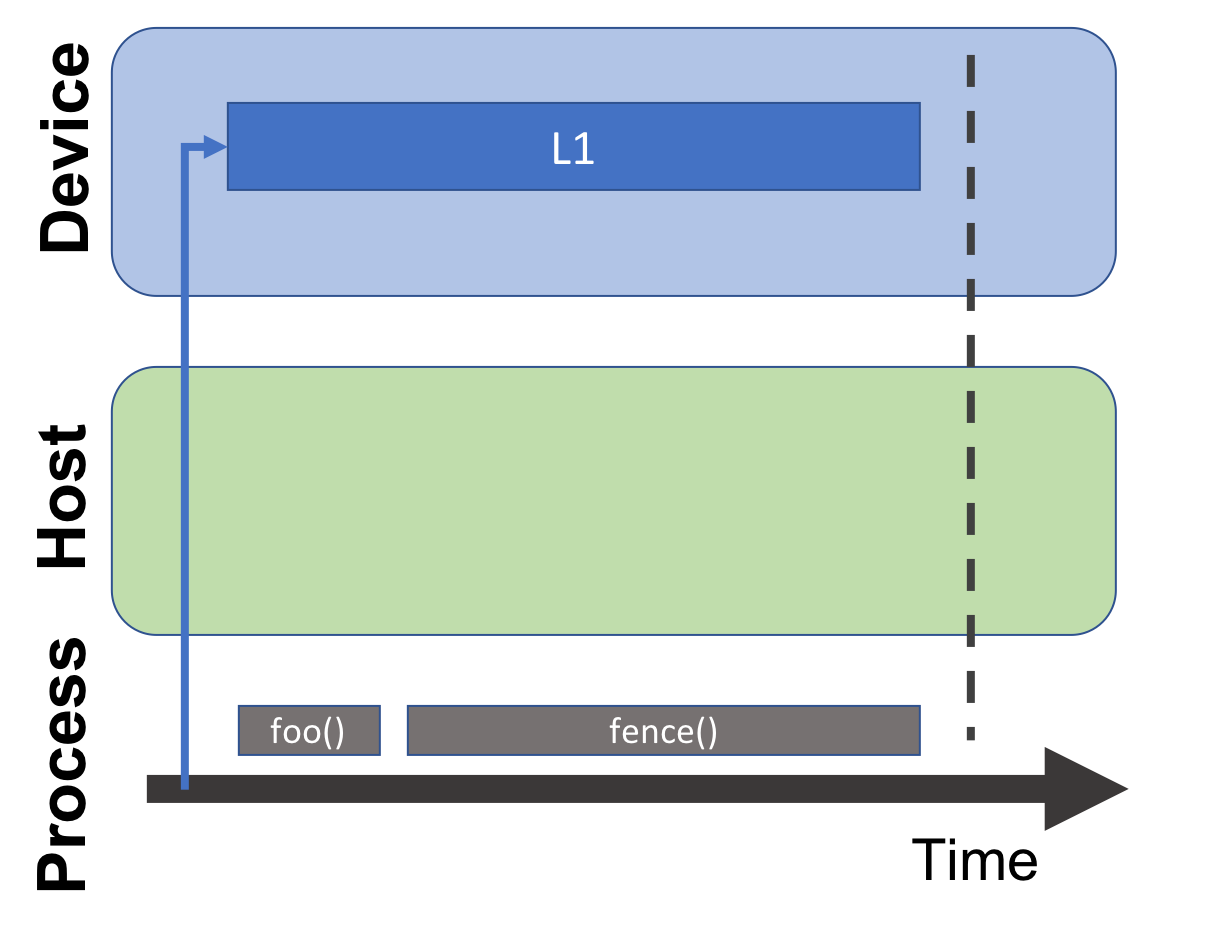
\includegraphics[width=0.95\textwidth]{figures/streams-fig0} 
 
    \end{column}

    \begin{column}{.33\textwidth}
	    \begin{code}[linebackgroundcolor={},keywords={L1,L2,policy_device}]
RangePolicy<> 
  policy_device(0,N)
FunctorL1 L1(...);

parallel_for("L1", 
  policy_device, L1);
foo();
fence();
      \end{code}
    \end{column}
  \end{columns}
\end{frame}
%==========================================================================

\begin{frame}[fragile]{Simple Dispatch}
  \textbf{Execution Spaces execute in dispatch order}
  \begin{itemize}
    \item{Dispatches to the same space instance will never overlap}
    \item{Executed in order FIFO}
    \item{Use \texttt{Kokkos::fence()} to wait for completion}
  \end{itemize}

  \begin{columns}[]
    \begin{column}{.67\textwidth}

       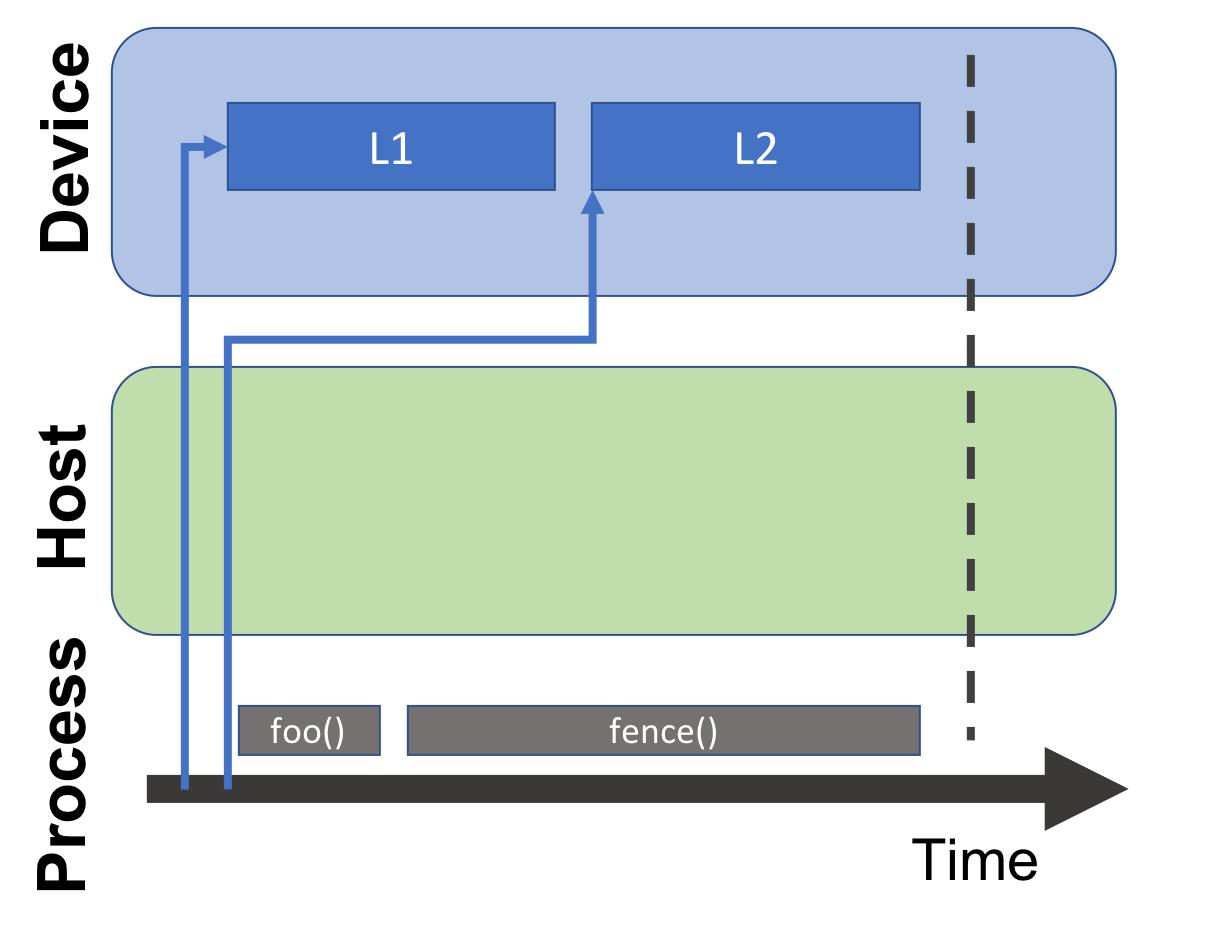
\includegraphics[width=0.95\textwidth]{figures/streams-fig1} 
 
    \end{column}

    \begin{column}{.33\textwidth}
	    \begin{code}[linebackgroundcolor={},keywords={L1,L2,policy_device}]
RangePolicy<> 
  policy_device(0,N)
FunctorL1 L1(...);
FunctorL2 L2(...);

parallel_for("L1", 
  policy_device, L1);
parallel_for("L2", 
  policy_device, L2);
foo();
fence();
      \end{code}
    \end{column}
  \end{columns}
\end{frame}

%==========================================================================

\begin{frame}[fragile]{Simple Dispatch}
  \textbf{Execution Spaces execute in dispatch order}
  \begin{itemize}
    \item{Dispatches to the same space instance will never overlap}
    \item{Executed in order FIFO}
    \item{Use \texttt{Kokkos::fence()} to wait for completion}
  \end{itemize}

  \begin{columns}[]
    \begin{column}{.67\textwidth}

       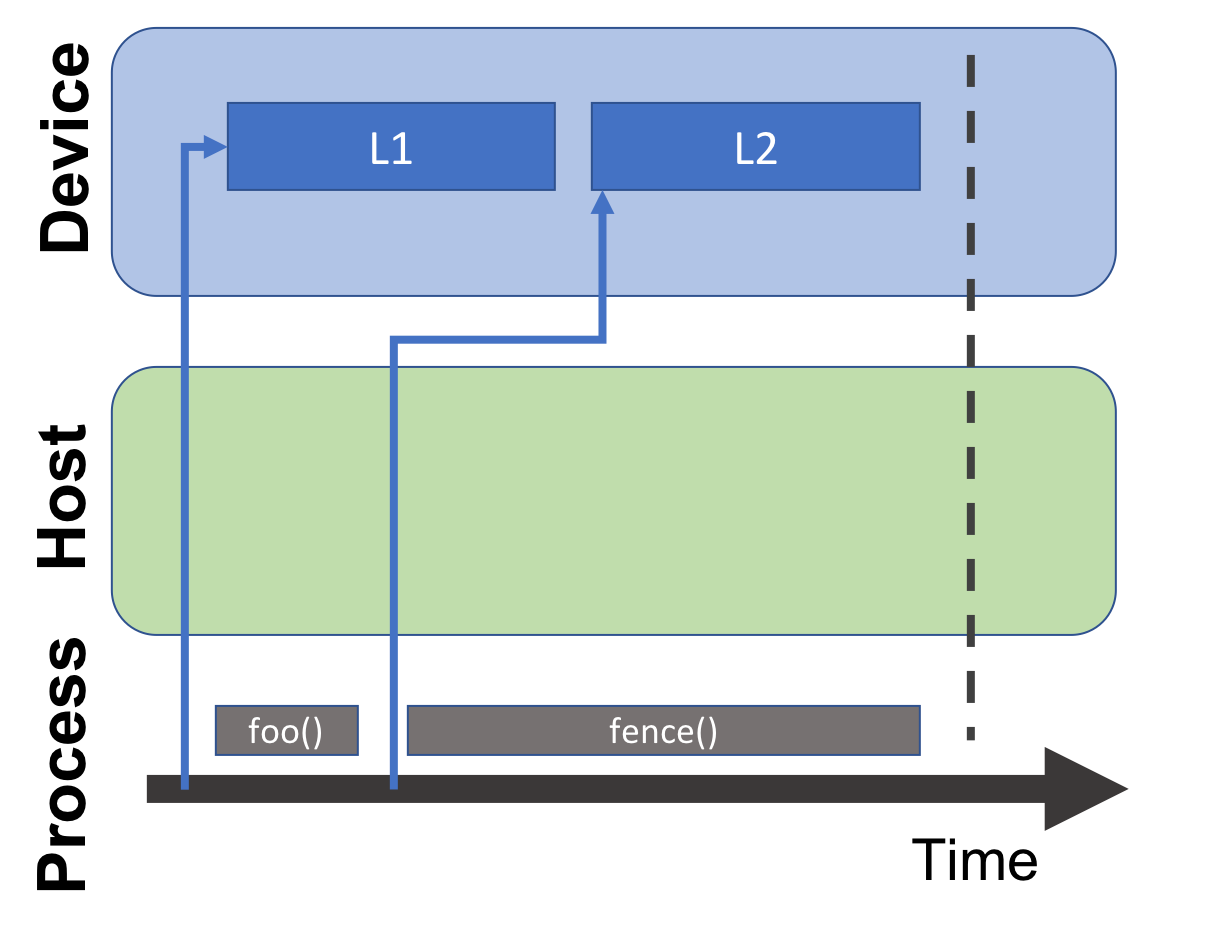
\includegraphics[width=0.95\textwidth]{figures/streams-fig2} 
 
    \end{column}

    \begin{column}{.33\textwidth}
	    \begin{code}[linebackgroundcolor={\btLstHL{8}{black!15}},keywords={L1,L2,policy_device}]
RangePolicy<> 
  policy_device(0,N)
FunctorL1 L1(...);
FunctorL2 L2(...);

parallel_for("L1", 
  policy_device, L1);
foo();
parallel_for("L2", 
  policy_device, L2);
fence();
      \end{code}
    \end{column}
  \end{columns}
\end{frame}

%==========================================================================

\begin{frame}[fragile]{Host/Device Dispatch}
  \textbf{ExecutionSpaces are Independent}
  \begin{itemize}
    \item{Dispatches into different ExecutionSpaces may overlap.}
    \item{Overlap with process thread functions and each other}
    \item{Use \texttt{Kokkos::fence()} to wait for completion of all}
  \end{itemize}

  \begin{columns}[]
    \begin{column}{.67\textwidth}

       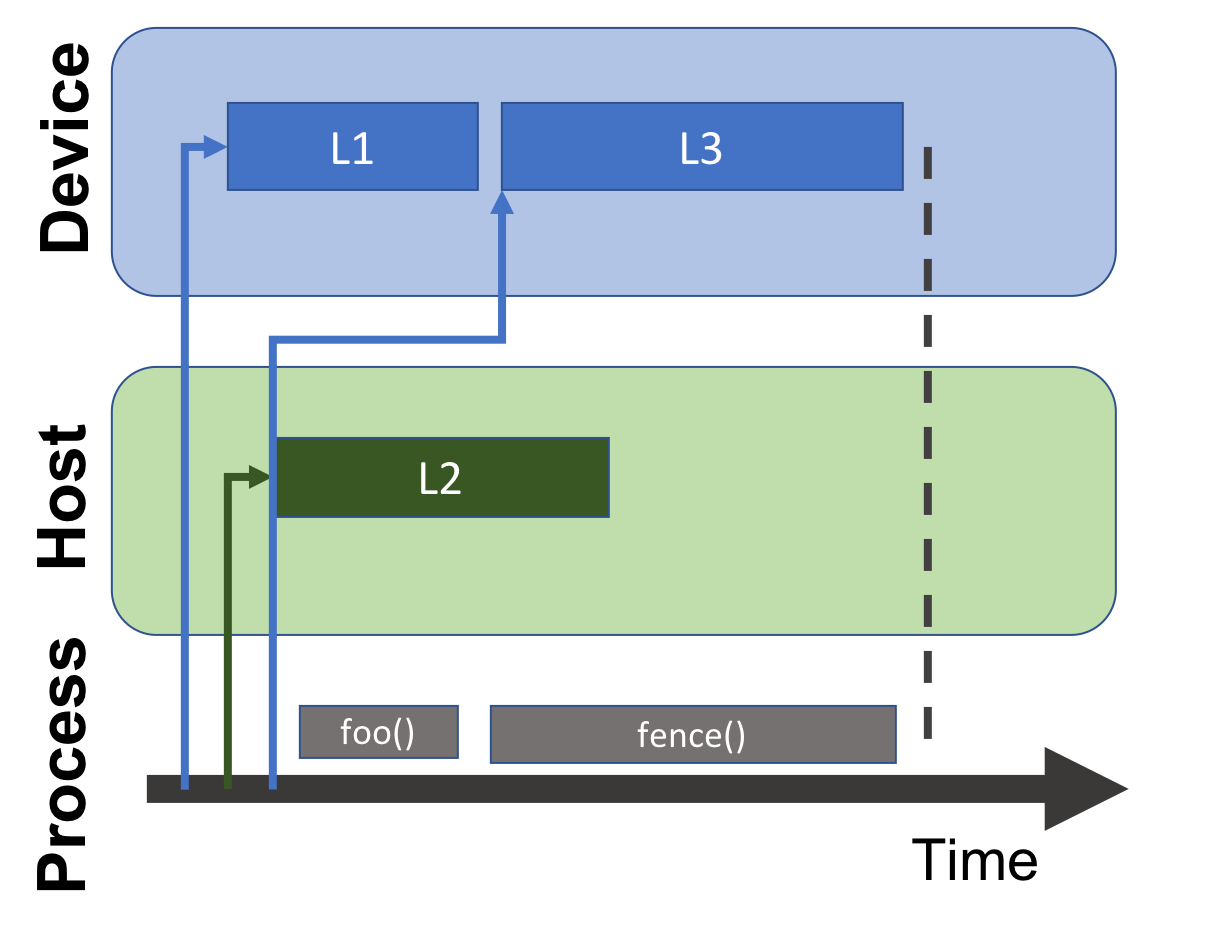
\includegraphics[width=0.95\textwidth]{figures/streams-fig3} 
 
    \end{column}

    \begin{column}{.33\textwidth}
	    \begin{code}[linebackgroundcolor={},keywords={L1,L2,L3,policy_device,policy_host}]
RangePolicy<> 
  policy_d(0,N)
RangePolicy<Host>
  policy_host(0,N)
FunctorL1 L1(...);
FunctorL2 L2(...);
FunctorL3 L3(...);
parallel_for("L1", 
  policy_d, L1);
parallel_for("L2", 
  policy_host, L2);
parallel_for("L3", 
  policy_d, L3);
foo();
fence();
      \end{code}
    \end{column}
  \end{columns}
\end{frame}

%==========================================================================

\begin{frame}[fragile]{Host/Device Dispatch Reality}
  \textbf{Reality: Some Host Backends Block}
  \begin{itemize}
  \item{Most host backends are blocking dispatches (except HPX)}
    \item{They never overlap with process thread functions}
    \item{But: \textbf{Do NOT rely on blocking behavior!!}}
  \end{itemize}

  \begin{columns}[]
    \begin{column}{.67\textwidth}

       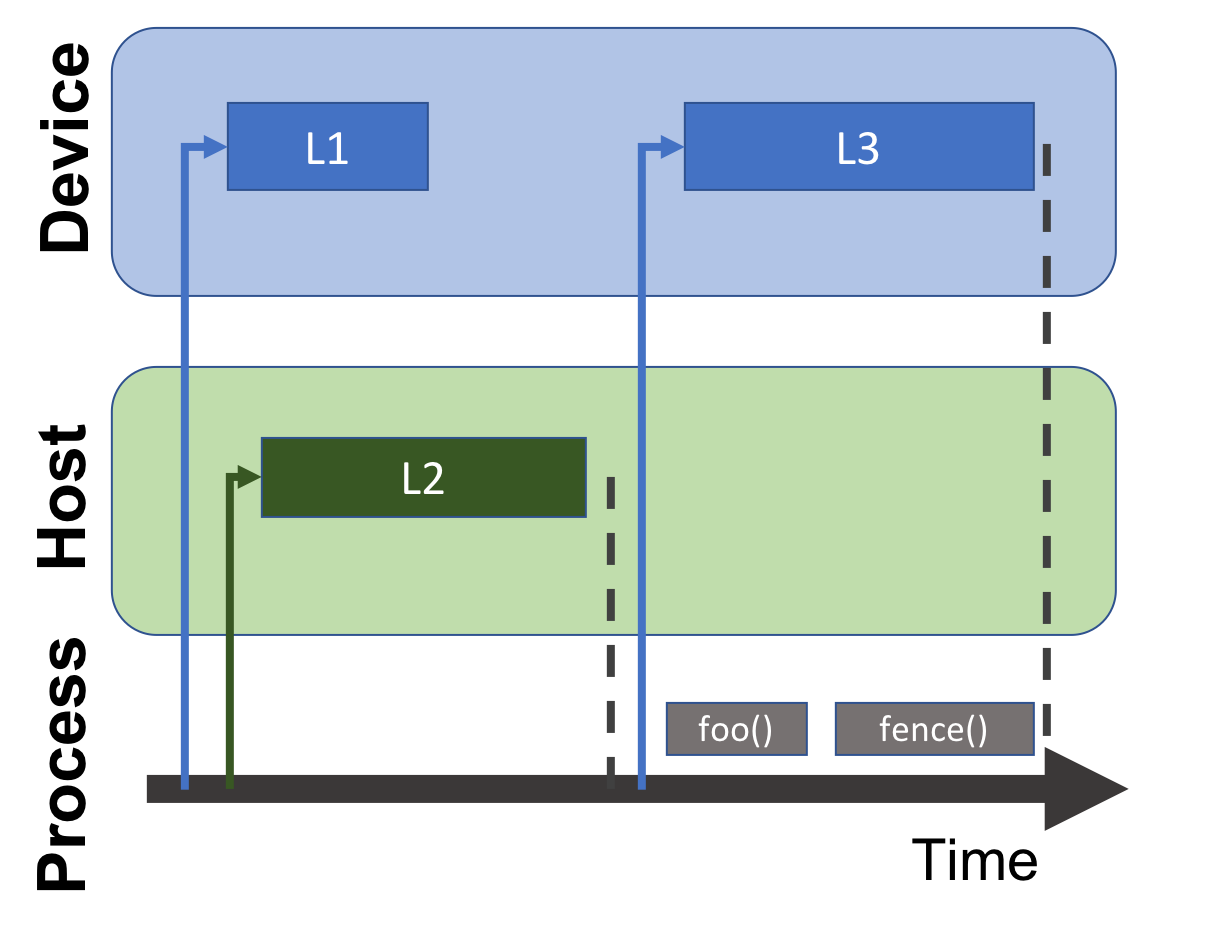
\includegraphics[width=0.95\textwidth]{figures/streams-fig4} 
 
    \end{column}

    \begin{column}{.33\textwidth}
	    \begin{code}[linebackgroundcolor={},keywords={L1,L2,L3,policy_device,policy_host}]
RangePolicy<> 
  policy_d(0,N)
RangePolicy<Host>
  policy_host(0,N)
FunctorL1 L1(...);
FunctorL2 L2(...);
FunctorL3 L3(...);
parallel_for("L1", 
  policy_d, L1);
parallel_for("L2", 
  policy_host, L2);
parallel_for("L3", 
  policy_d, L3);
foo();
fence();
      \end{code}
    \end{column}
  \end{columns}
\end{frame}

%==========================================================================

\begin{frame}[fragile]{Reductions}
  \textbf{Reductions to Scalars are Blocking}
  \begin{itemize}
    \item{The call only returns after result is available.}
    \item{FIFO implies, every other kernel in the same ExecutionSpace instance will be done too}
  \end{itemize}

  \begin{columns}[]
    \begin{column}{.67\textwidth}

       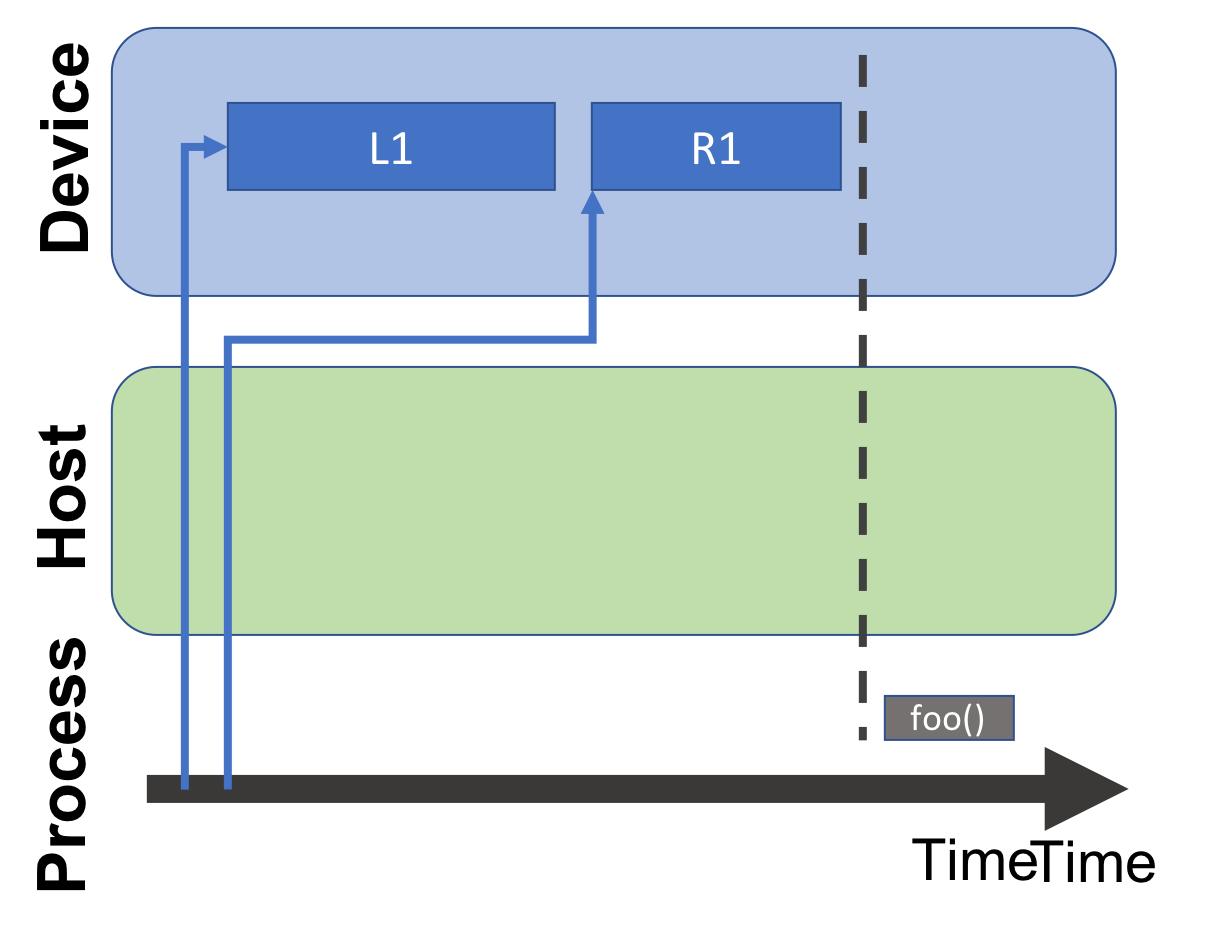
\includegraphics[width=0.95\textwidth]{figures/streams-fig5} 
 
    \end{column}

    \begin{column}{.33\textwidth}
	    \begin{code}[linebackgroundcolor={},keywords={L1,L2,policy_device}]
RangePolicy<> 
  policy_d(0,N)
FunctorL1 L1(...);
FunctorR1 R1(...);

double result;
parallel_for("L1", 
  policy_d, L1);
parallel_reduce("R1", 
  policy_d, R1, result);
foo();
      \end{code}
    \end{column}
  \end{columns}
\end{frame}

%==========================================================================

\begin{frame}[fragile]{Reductions to Scalars}
  \textbf{Reductions to Scalars are Blocking}
  \begin{itemize}
    \item{The call only returns after result is available.}
    \item{For subsequent dispatches previous rules apply}
  \end{itemize}

  \begin{columns}[]
    \begin{column}{.67\textwidth}

       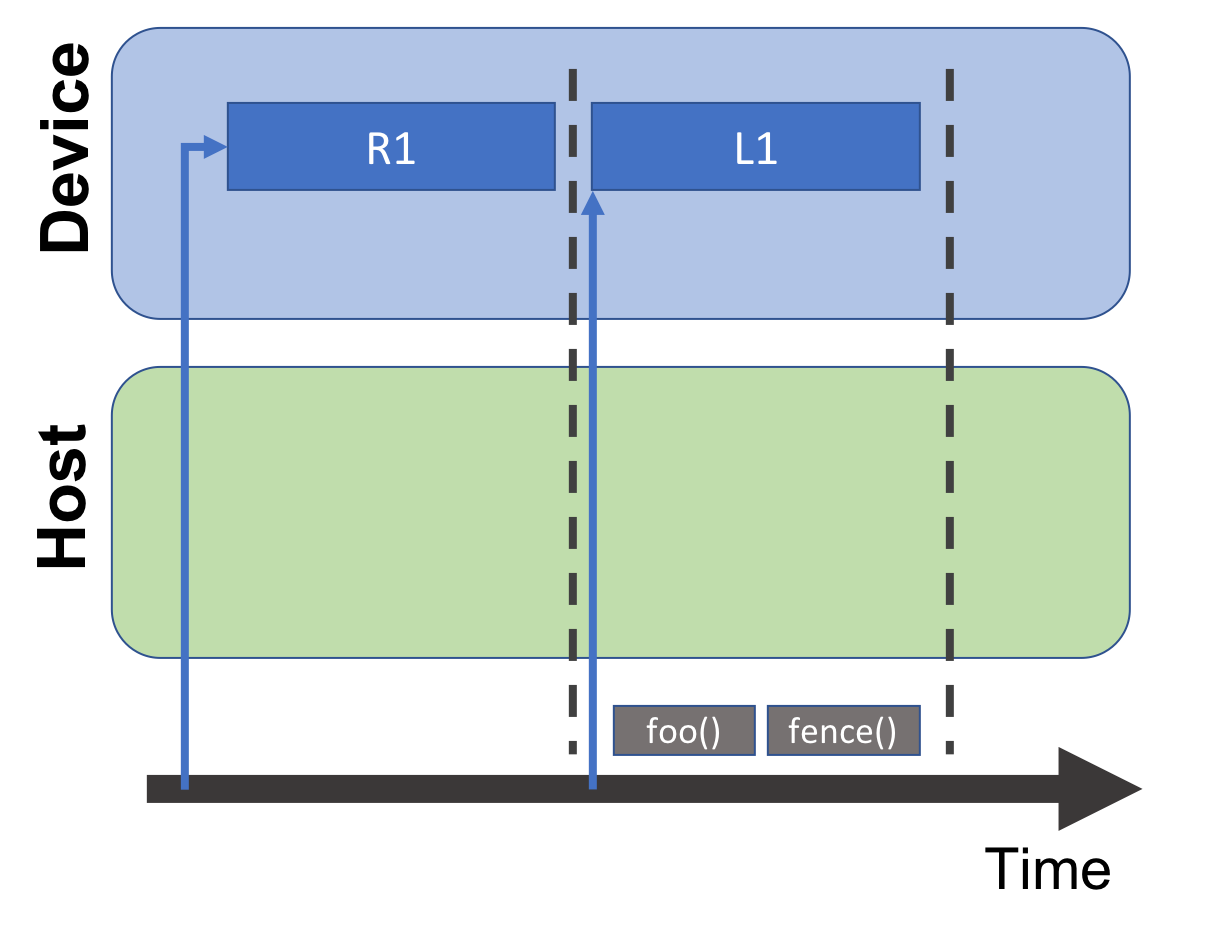
\includegraphics[width=0.95\textwidth]{figures/streams-fig6} 
 
    \end{column}

    \begin{column}{.33\textwidth}
	    \begin{code}[linebackgroundcolor={},keywords={L1,L2,policy_device}]
RangePolicy<> 
  policy_d(0,N)
FunctorL1 L1(...);
FunctorR1 R1(...);

double result;
parallel_reduce("R1", 
  policy_d, R1, result);
parallel_for("L1", 
  policy_d, L1);
foo();
fence();
      \end{code}
    \end{column}
  \end{columns}
\end{frame}

%==========================================================================

\begin{frame}[fragile]{Reductions to Views}
  \textbf{Reductions to Views are Non-blocking}
  \begin{itemize}
    \item{Behave like a \texttt{parallel\_for}}
    \item{Results are only available after a \texttt{Kokkos::fence()}}
    \item{Even true for unmanaged \texttt{View}s of host variables!}
  \end{itemize}

  \begin{columns}[]
    \begin{column}{.67\textwidth}

       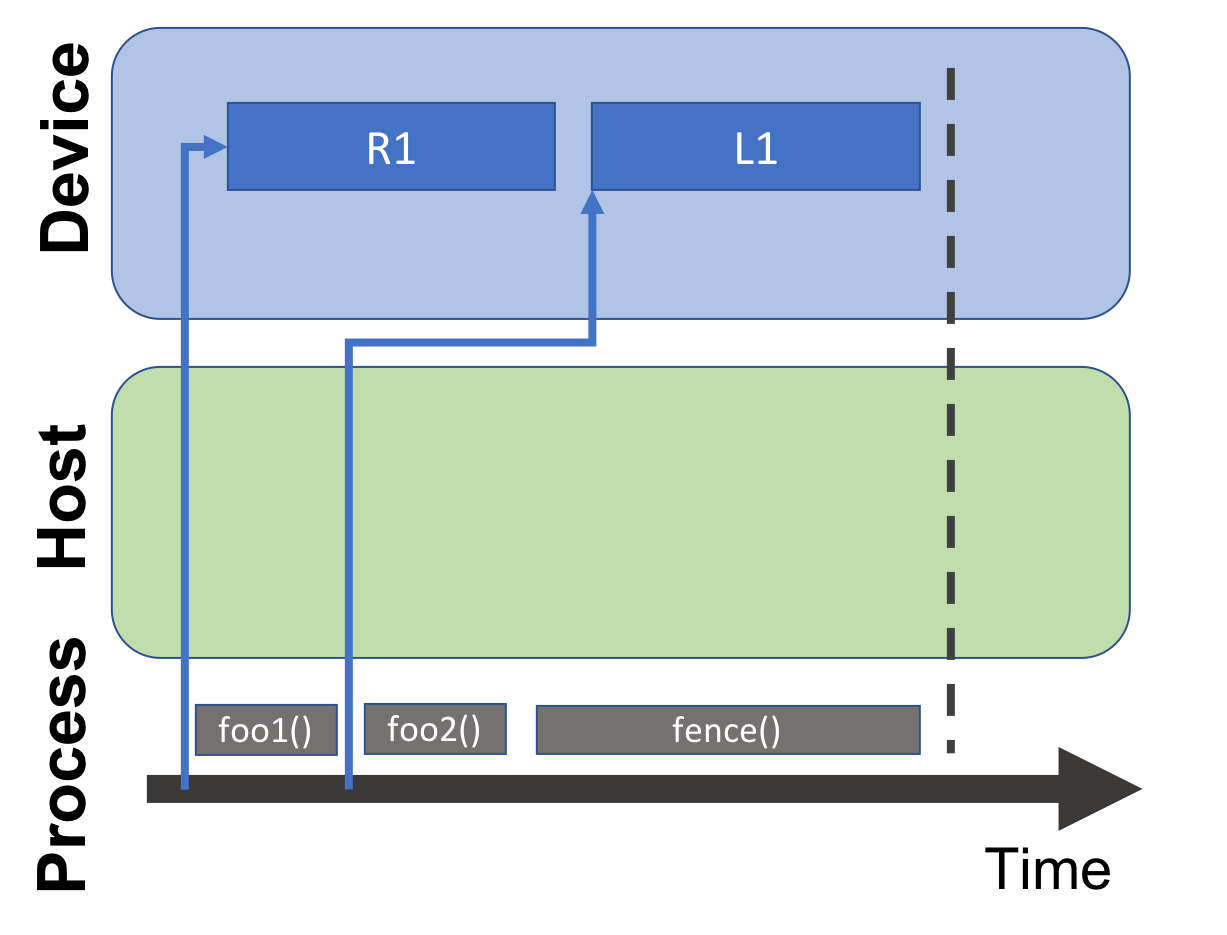
\includegraphics[width=0.95\textwidth]{figures/streams-fig7} 
 
    \end{column}

    \begin{column}{.33\textwidth}
    \begin{code}[linebackgroundcolor={},keywords={L1,L2,policy_device}]
...
double result;
View<double, HostSpace>
  v_result(&result);
parallel_reduce("R1", 
  policy_d,R1,v_result);
foo1();
parallel_for("L1", 
  policy_d, L1);
foo2();
fence();
      \end{code}
    \end{column}
  \end{columns}
\end{frame}

%==========================================================================

\begin{frame}[fragile]{Simple Dispatch}
  \textbf{Simple Parallel Loop}
  \begin{itemize}
    \item{Asynchronous}
    \item{Overlaps with host functions}
    \item{Use \texttt{Kokkos::fence()} to wait for completion}
  \end{itemize}

  \begin{columns}[]
    \begin{column}{.67\textwidth}

       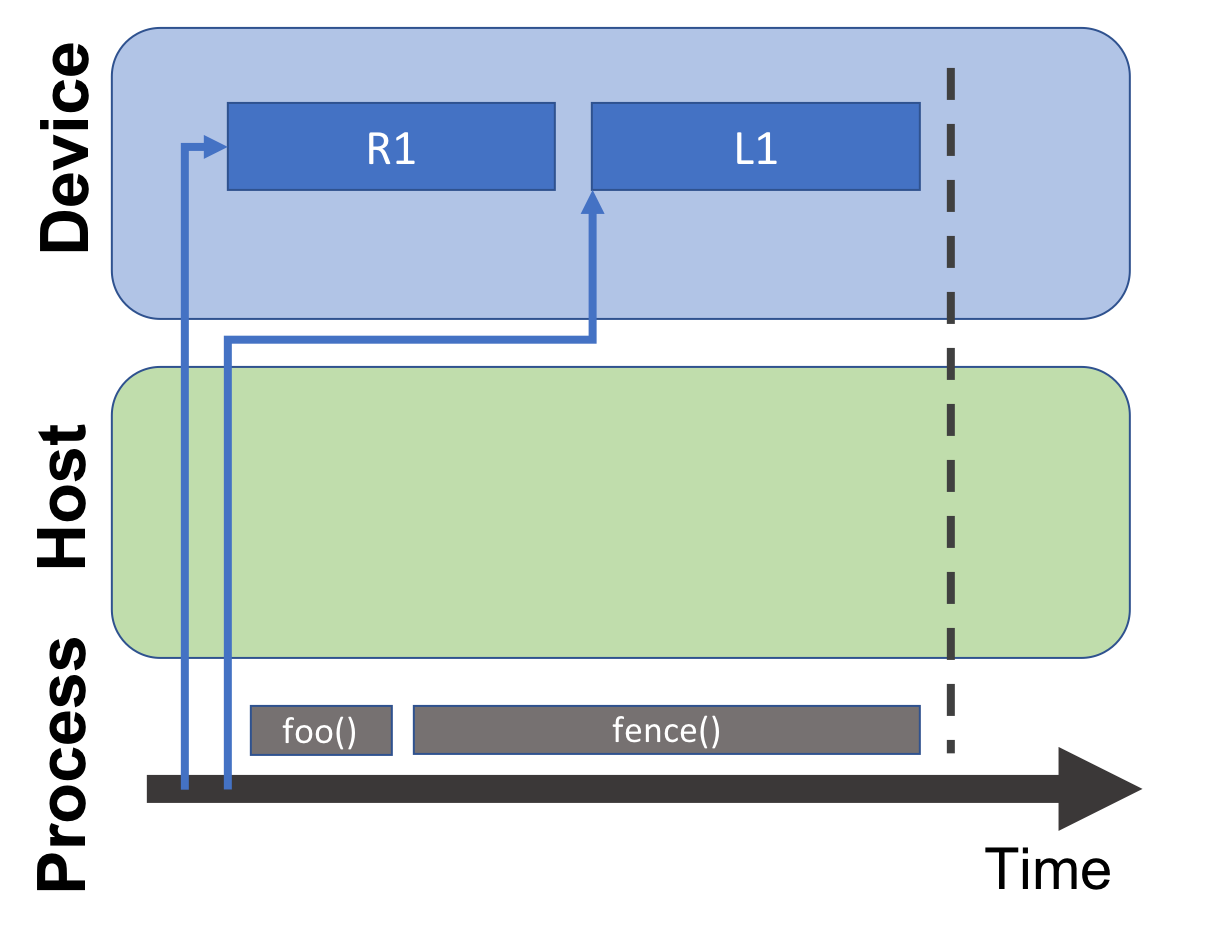
\includegraphics[width=0.95\textwidth]{figures/streams-fig8} 
 
    \end{column}

    \begin{column}{.33\textwidth}
	    \begin{code}[linebackgroundcolor={},keywords={L1,L2,policy_device}]
RangePolicy<> 
  policy_device(0,N)
FunctorL1 L1(...);
FunctorL2 L2(...);

parallel_for("L1", 
  policy_device, L1);
parallel_for("L2", 
  policy_device, L2);
foo();
fence();
      \end{code}
    \end{column}
  \end{columns}
\end{frame}

%==========================================================================

\begin{frame}[fragile]{Deep Copy}
  \textbf{2-Argument deep\_copy is fully blocking}
  \begin{itemize}
    \item{Implies a full \texttt{fence} before the copy}
    \item{Copy is done by the time call returns.}
    \item{Even if it is a no-op due to \texttt{src == dst}!}
  \end{itemize}

  \begin{columns}[]
    \begin{column}{.67\textwidth}

       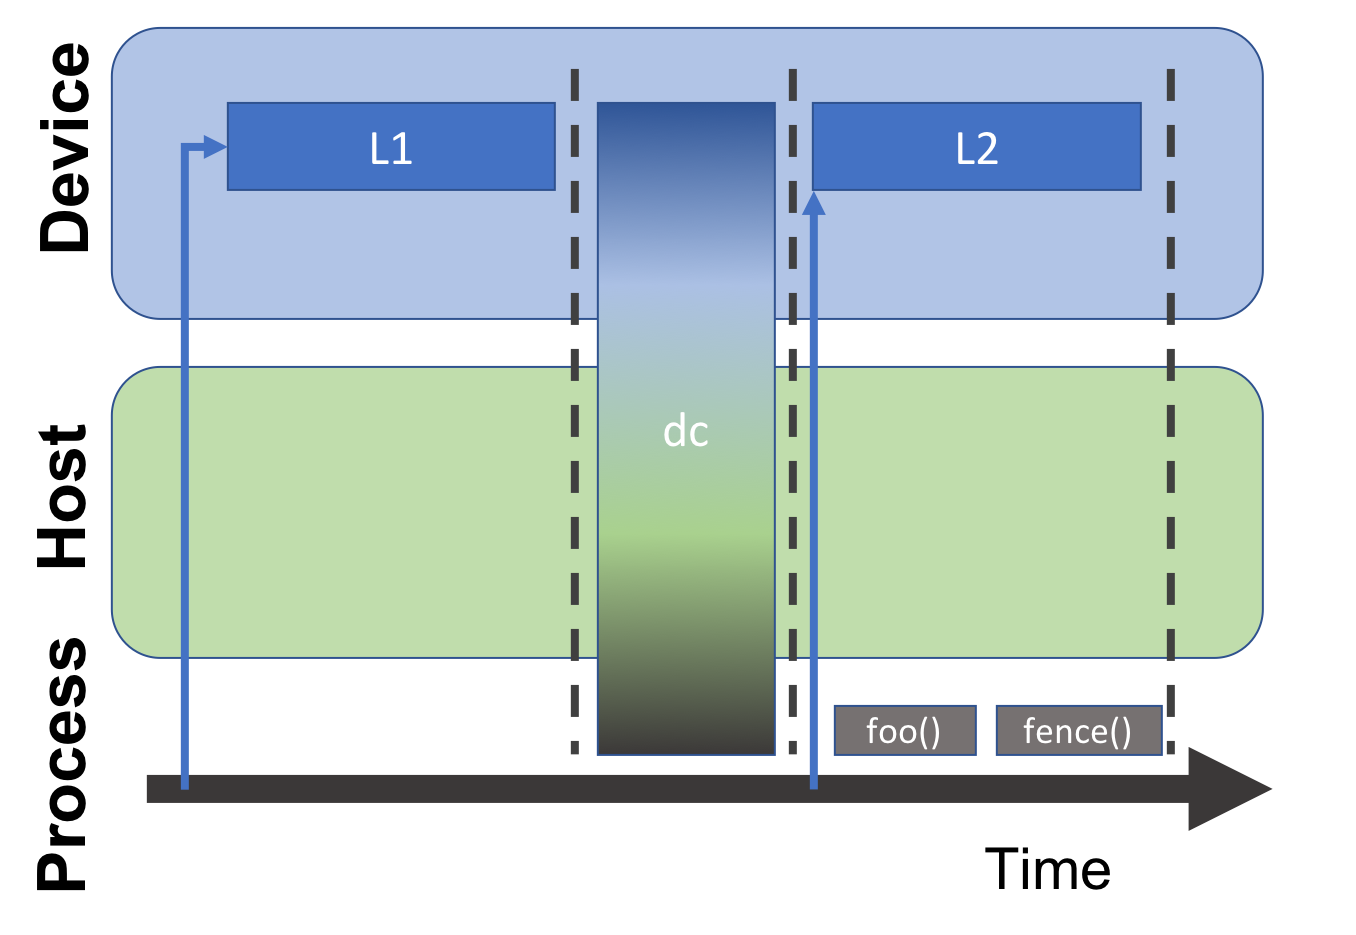
\includegraphics[width=0.95\textwidth]{figures/streams-fig9} 
 
    \end{column}

    \begin{column}{.33\textwidth}
	    \begin{code}[linebackgroundcolor={},keywords={L1,L2,policy_device}]

parallel_for("L1", 
  policy_device, L1);
deep_copy(dest,src);
parallel_for("L2", 
  policy_device, L2);
foo();
fence();
      \end{code}
    \end{column}
  \end{columns}
\end{frame}

%==========================================================================

\begin{frame}[fragile]{Deep Copy}
  \textbf{deep\_copy with space argument are non-blocking}
  \begin{itemize}
    \item{Execute in dispatch order in the queue of the space}
    \item{Overlap with host process functions}
    \item{Use \texttt{Kokkos::fence()} to wait for completion}
  \end{itemize}

  \begin{columns}[]
    \begin{column}{.67\textwidth}

       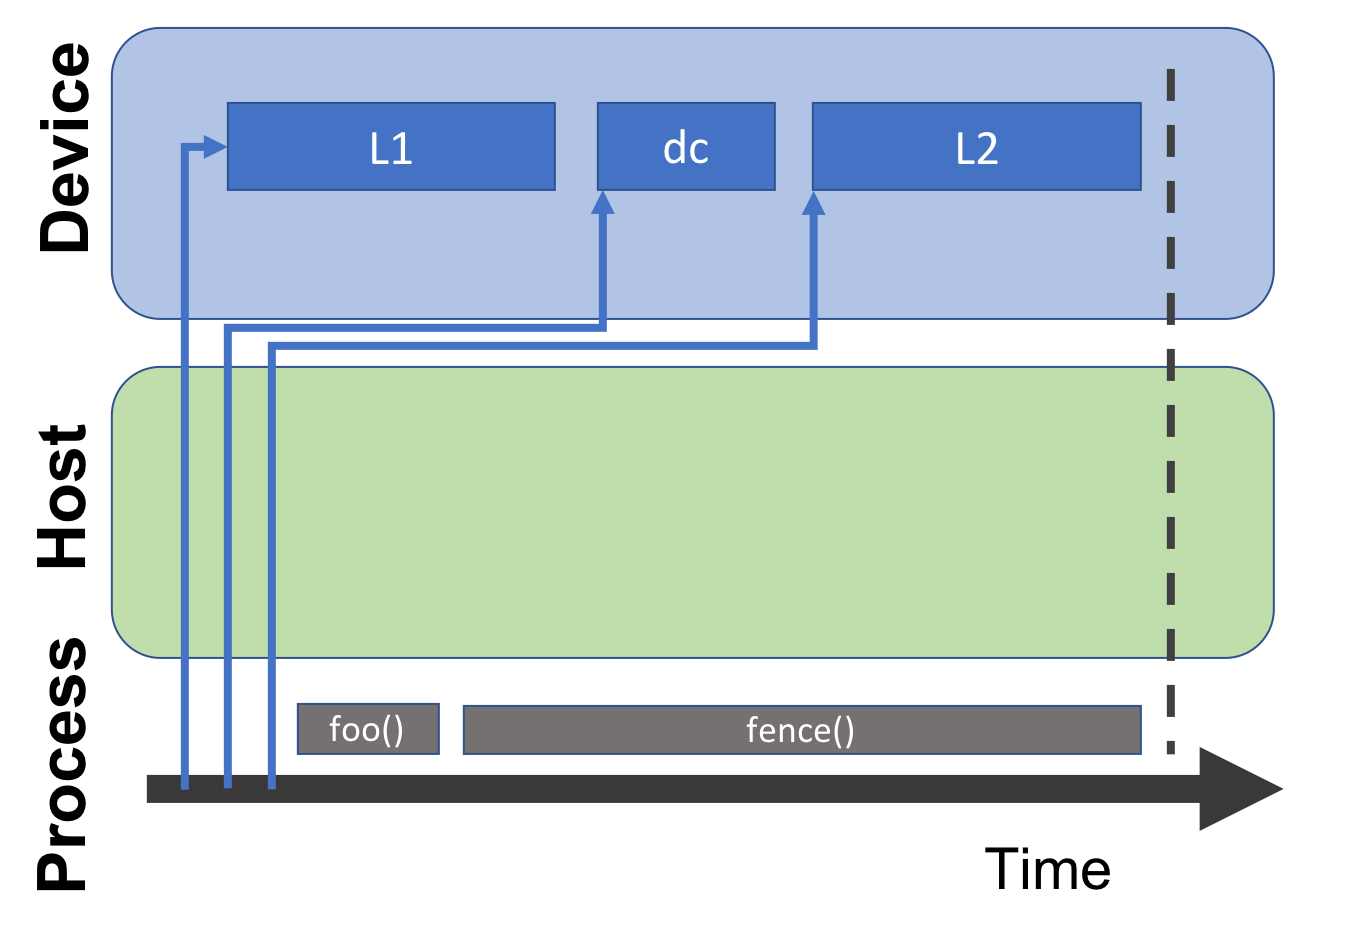
\includegraphics[width=0.95\textwidth]{figures/streams-fig10} 
 
    \end{column}

    \begin{column}{.33\textwidth}
	    \begin{code}[linebackgroundcolor={},keywords={L1,L2,policy_device}]
parallel_for("L1", 
  policy_device, L1);
deep_copy(device,
  dest,src);
parallel_for("L2", 
  policy_device, L2);
foo();
fence();
      \end{code}
    \end{column}
  \end{columns}
\end{frame}

%==========================================================================

\begin{frame}[fragile]{Deep Copy}
  \textbf{deep\_copy with space argument are non-blocking}
  \begin{itemize}
    \item{Execute in dispatch order in the queue of the space}
    \item{Overlap with other execution spaces}
    \item{Use \texttt{Kokkos::fence()} to wait for completion}
  \end{itemize}

  \begin{columns}[]
    \begin{column}{.67\textwidth}

       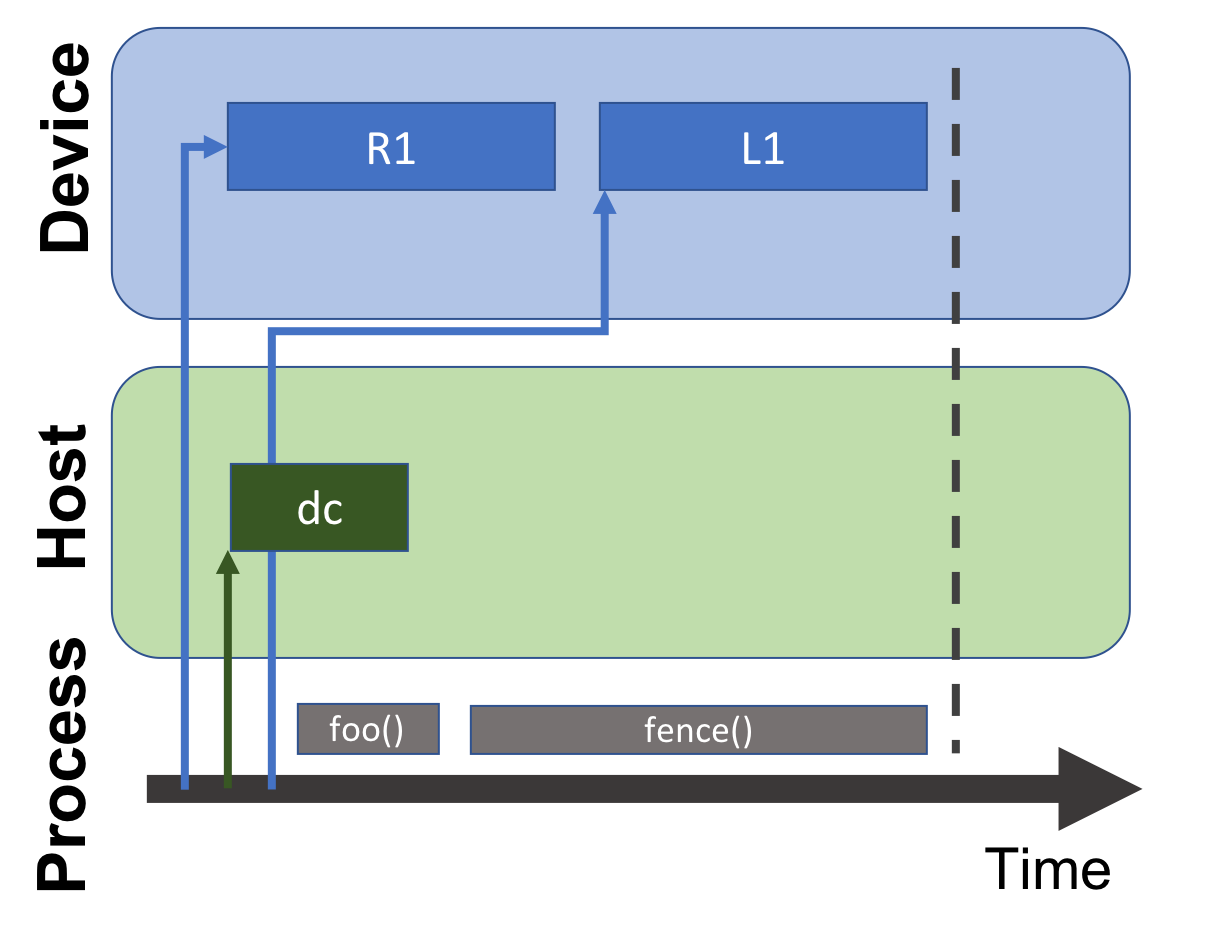
\includegraphics[width=0.95\textwidth]{figures/streams-fig11} 
 
    \end{column}

    \begin{column}{.33\textwidth}
	    \begin{code}[linebackgroundcolor={},keywords={L1,L2,policy_device}]
parallel_for("L1", 
  policy_device, L1);
deep_copy(host(),
  dest,src);
parallel_for("L2", 
  policy_device, L2);
foo();
fence();
      \end{code}
    \end{column}
  \end{columns}
\end{frame}

%==========================================================================

\begin{frame}[fragile]{Multiple Instances}
  \textbf{So what about CUDA streams?}

	Up to now we only used default execution space instances, but what if you want to have concurrent kernels on the GPU?

	\pause
	\begin{block}{Execution Space Instances}
		Execution Space instances behave largely like CUDA streams
	\end{block}

	\pause
	You can create different instances:
	\begin{itemize}
		\item Fairly new capability. 
		\item Initial version more for interoperability with CUDA/HIP.
		\begin{itemize}
			\item Give a \texttt{cudaStream\_t} to the constructor of the instance:
				\begin{code}[]
	cudaStream_t stream = ...;
	Kokkos::Cuda cuda_instance(stream);
				\end{code}
		\end{itemize}
		\item Generic versions upcoming (e.g. create generic instances)
		\item Not all spaces support having multiple distinct instances.
		\item ExecutionSpace instances are like shared pointers. 
	\end{itemize}

\end{frame}

%==========================================================================

\begin{frame}[fragile]{Multiple Instances}
  \textbf{Instances of Execution Spaces own a exec queue}
  \begin{itemize}
    \item{Work dispatched to different instances overlaps with each other}
    \item{Overlaps with host process functions}
    \item{Use \texttt{Kokkos::fence()} to wait for completion of all}
  \end{itemize}

  \begin{columns}[]
    \begin{column}{.67\textwidth}

       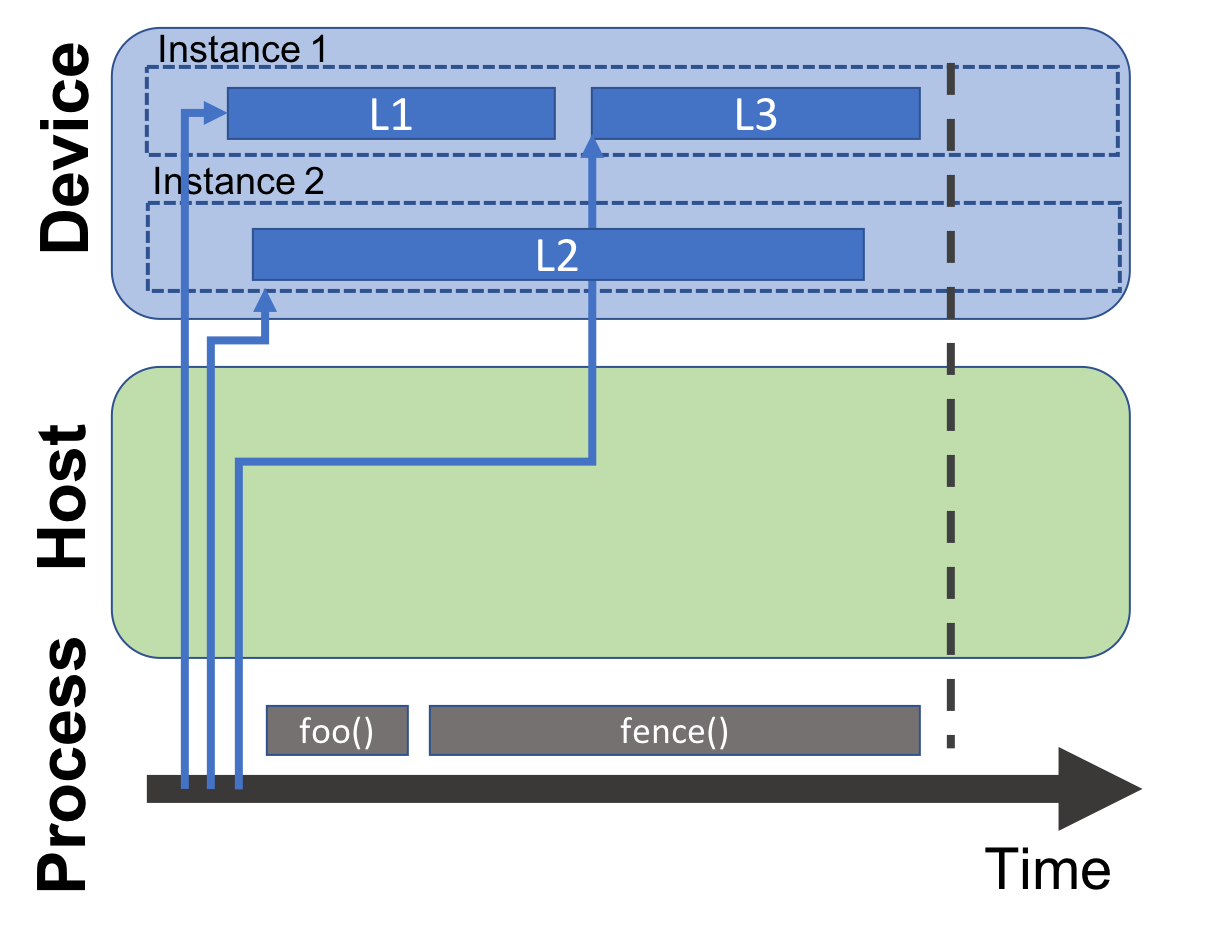
\includegraphics[width=0.95\textwidth]{figures/streams-fig12} 
 
    \end{column}

    \begin{column}{.33\textwidth}
	    \begin{code}[linebackgroundcolor={},keywords={L1,L2,policy_device}]
Device dev1(...);
Device dev2(...);
RangePolicy<Device>
  policy_d1(dev1,0,N);
RangePolicy<Device>
  policy_d2(dev2,0,N);

parallel_for("L1", 
  policy_d1, L1);
parallel_for("L2", 
  policy_d2, L2);
parallel_for("L3", 
  policy_d1, L3);
foo();
fence();
      \end{code}
    \end{column}
  \end{columns}
\end{frame}

%==========================================================================

\begin{frame}[fragile]{Multiple Instances}
  \textbf{deep\_copy with an instance argument also overlap}
  \begin{itemize}
    \item{deep\_copy with an instance argument are like any other parallel operation}
    \item{Overlaps with parallel operations in other instance}
  \end{itemize}

  \begin{columns}[]
    \begin{column}{.67\textwidth}

       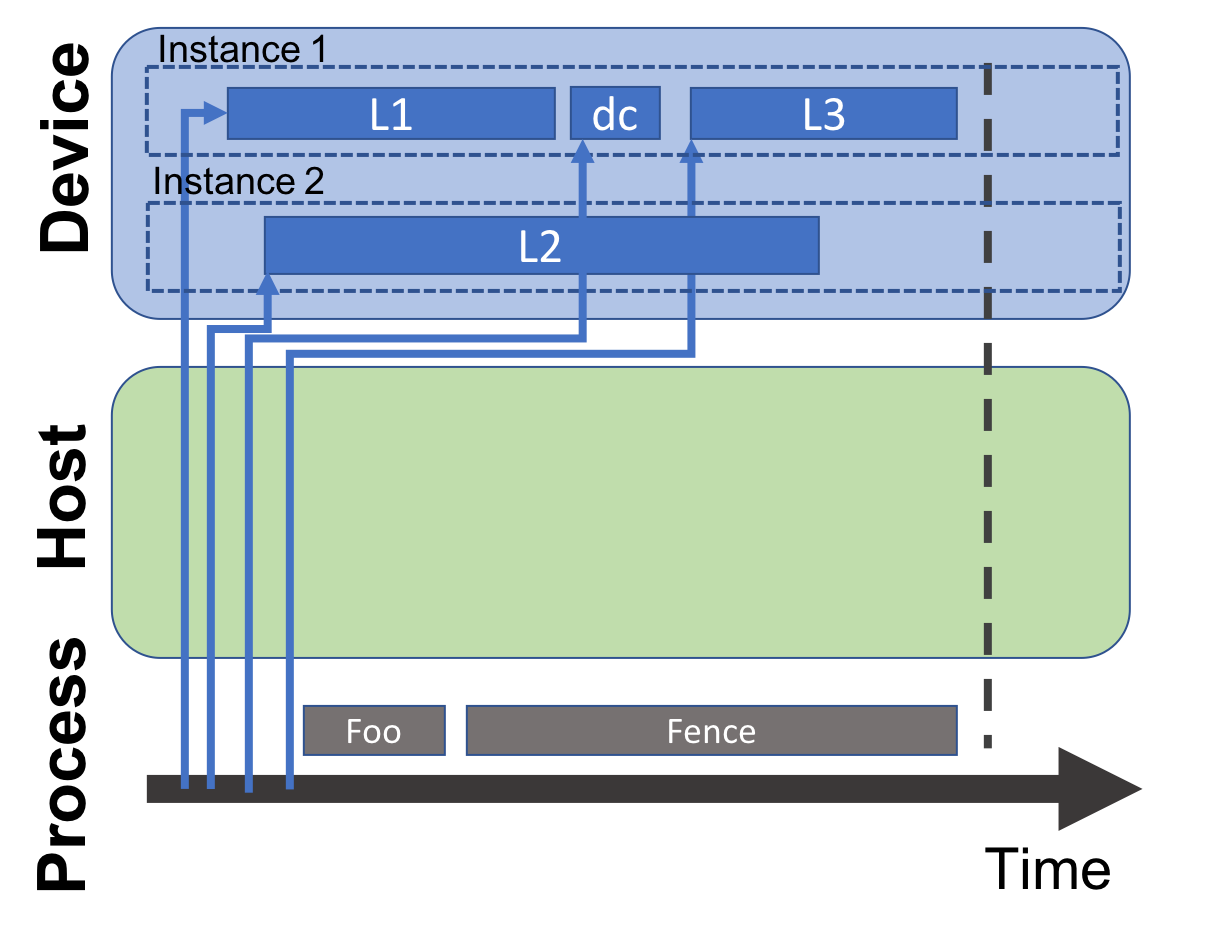
\includegraphics[width=0.95\textwidth]{figures/streams-fig13} 
 
    \end{column}

    \begin{column}{.33\textwidth}
	    \begin{code}[linebackgroundcolor={},keywords={L1,L2,policy_device}]
parallel_for("L1", 
  policy_d1, L1);
parallel_for("L2", 
  policy_d2, L2);
deep_copy(dev1,
  dest, src);
parallel_for("L3", 
  policy_d1, L3);
foo();
fence();
      \end{code}
    \end{column}
  \end{columns}
\end{frame}

%==========================================================================

\begin{frame}[fragile]{Fencing}
	\textbf{There are instance fences}
  \begin{itemize}
    \item{Use instance specific fence to only wait on that instance}
    \item{Operations in other instances can overlap with that fence}
    \item{Use \texttt{Kokkos::fence()} to wait for all outstanding ops}
  \end{itemize}

  \begin{columns}[]
    \begin{column}{.67\textwidth}

       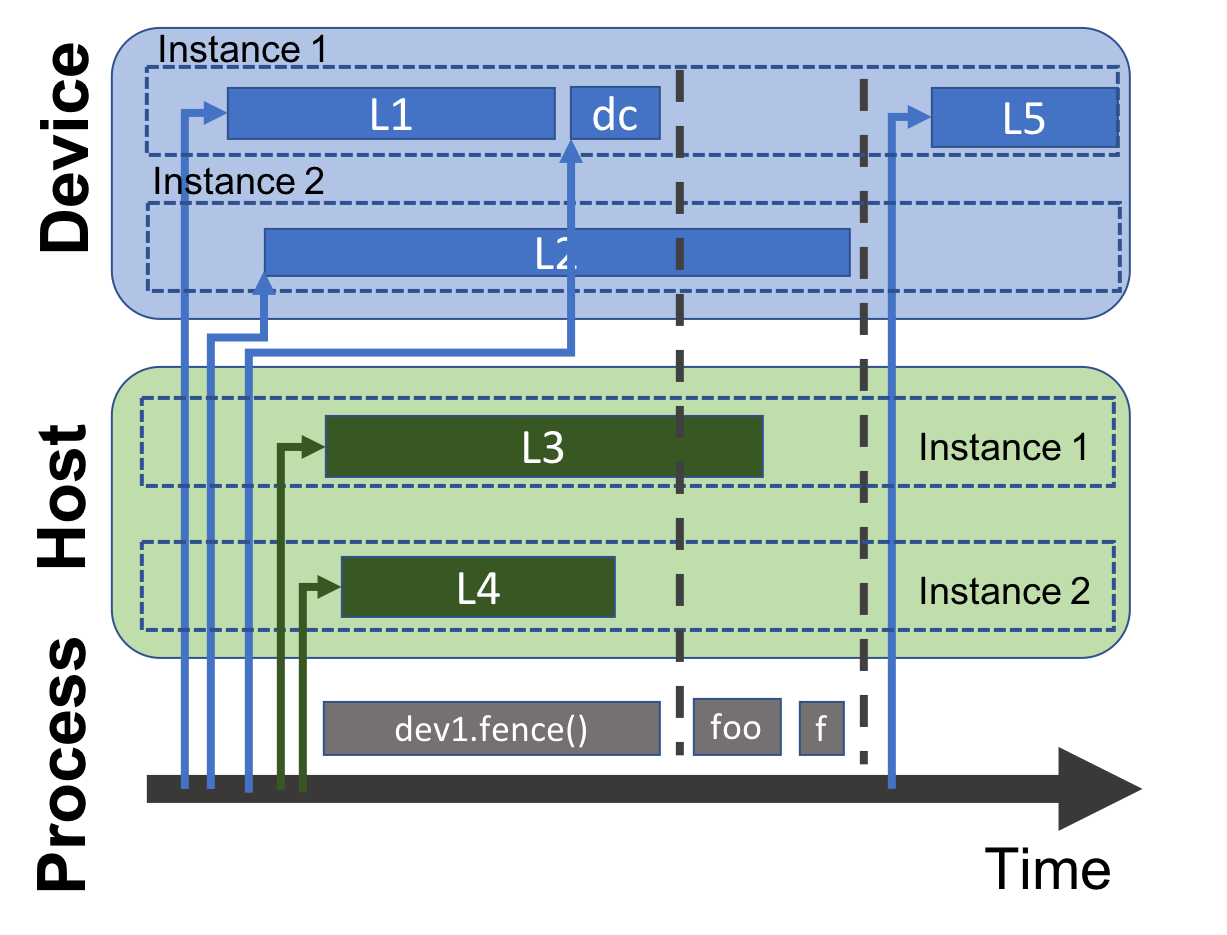
\includegraphics[width=0.95\textwidth]{figures/streams-fig14} 
 
    \end{column}

    \begin{column}{.33\textwidth}
	    \begin{code}[linebackgroundcolor={},keywords={L1,L2,policy_device}]
parallel_for("L1", 
  policy_d1, L1);
parallel_for("L2", 
  policy_d2, L2);
deep_copy(dev1,
  dest, src);
parallel_for("L3", 
  policy_h1, L3);
parallel_for("L4", 
  policy_h2, L4);
dev1.fence();
foo();
fence();
parallel_for("L5", 
  policy_d1, L5);
      \end{code}
    \end{column}
  \end{columns}
\end{frame}

%==========================================================================

\begin{frame}[fragile]{Deallocation}
	\textbf{Reality Check: Kokkos Views deallocation implies fence!}
  \begin{itemize}
    \item{Due to limitations of reference counting, deallocations fence!}
    \item{\textbf{Important:} this is implementation limitation not semantic!}
    \item{\textbf{Do NOT rely on deallocations fencing!}}
  \end{itemize}

  \begin{columns}[]
    \begin{column}{.67\textwidth}

       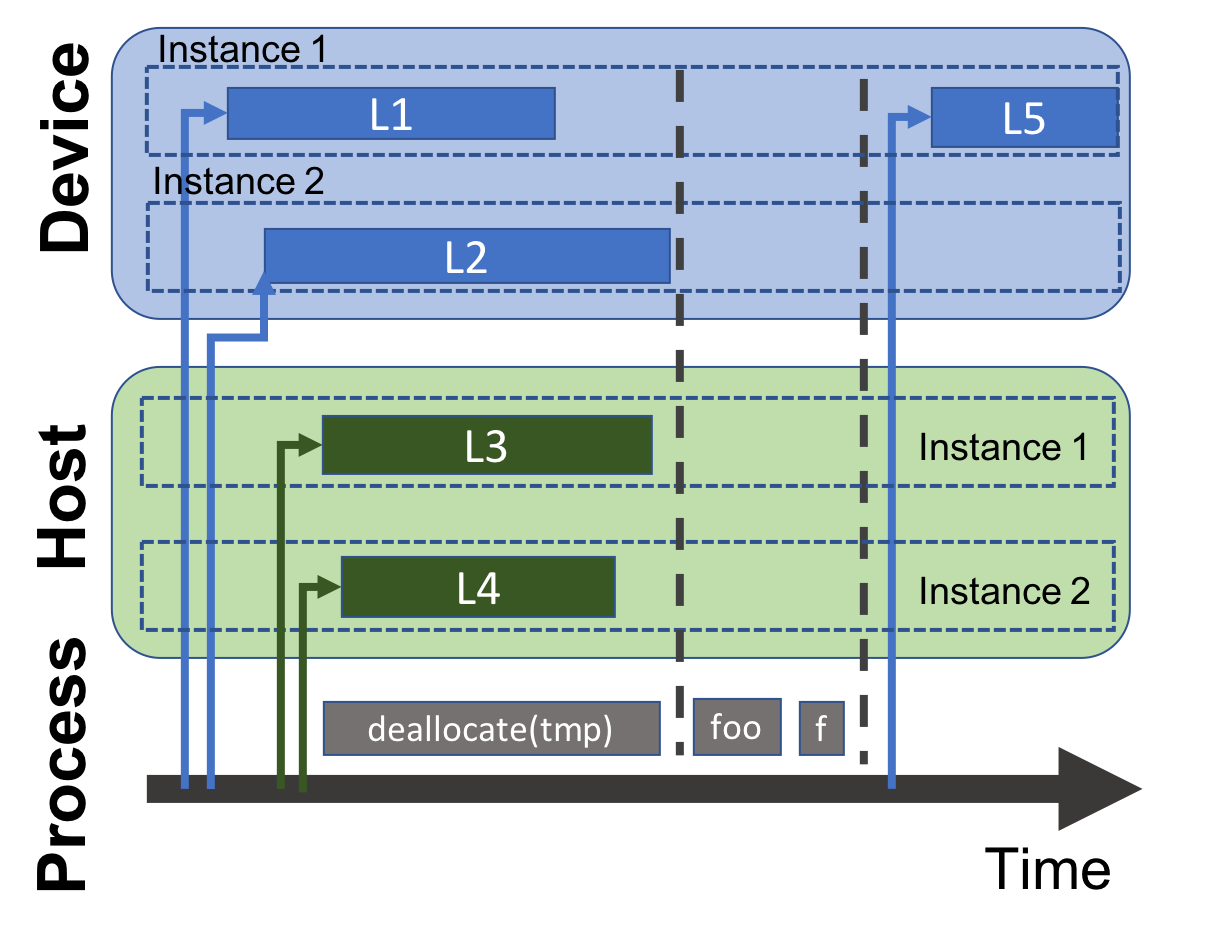
\includegraphics[width=0.95\textwidth]{figures/streams-fig15} 
 
    \end{column}

    \begin{column}{.33\textwidth}
	    \begin{code}[linebackgroundcolor={},keywords={L1,L2,policy_device}]
{
View<..> tmp(...);
parallel_for("L1", 
  policy_d1, L1);
parallel_for("L2", 
  policy_d2, L2);
parallel_for("L3", 
  policy_h1, L3);
parallel_for("L4", 
  policy_h2, L4);
}
foo();
fence();
parallel_for("L5", 
  policy_d1, L5);
      \end{code}
    \end{column}
  \end{columns}
\end{frame}


\begin{frame}{Section Summary}

  \begin{itemize}
    \item{Execution Space Instances execute work in order of dispatch.}
    \item{Operations dispatched to different Execution Space Instances can overlap.}
    \item{Each Execution Space type has a default instance as a singleton.}
    \item{Use \texttt{Kokkos::fence()} to wait for completion of ALL outstanding work.}
    \item{Use \texttt{exec\_space\_instance.fence()} to wait for completion of outstanding work dispatched to a specific execution space instance.}
  \end{itemize}

\end{frame}


%==========================================================================

\begin{frame}[fragile]

  {\Huge Task parallelism}

  \vspace{10pt}

  {\large Fine-grained dependent execution.}

  \vspace{20pt}

  \textbf{Learning objectives:}
  \begin{itemize}
    \item {Basic interface for fine-grained tasking in Kokkos}
    \item {How to express dynamic dependency structures in Kokkos tasking}
    \item {When to use Kokkos tasking}
  \end{itemize}

  \vspace{-20pt}

\end{frame}

%==========================================================================

\begin{frame}[fragile]{Task Parallelism Looks Like Data Parallelism}

    Recall that {\textbf{data parallel}} code is composed of a {\color{patternColor!80!black} pattern}, a {\color{policyColor!80!black} policy}, and a {\color{bodyColor!80!black} functor}

    \vspace{3pt}

    \begin{code}[linebackgroundcolor={},keywords={}]
@patternKokkos::parallel_for@pattern(
  @policyKokkos::RangePolicy<>(exec_space, 0, N)@policy,
  @bodySomeFunctor()@body
);
  \end{code}
    \vspace{8pt}

    \textbf{Task parallel} code similarly has a {\color{patternColor!80!black} pattern}, a {\color{policyColor!80!black} policy}, and a {\color{bodyColor!80!black} functor}

    \vspace{3pt}

    \begin{code}[linebackgroundcolor={},keywords={}]
@patternKokkos::task_spawn@pattern(
  @policyKokkos::TaskSingle(scheduler, TaskPriority::High)@policy,
  @bodySomeFunctor()@body
);
    \end{code}
\end{frame}

%==========================================================================

\begin{frame}[fragile]{What does a task functor look like?}

  \begin{code}[linebackgroundcolor={},keywords={}]
struct MyTask {
  using @bluevalue_type@blue = @reddouble@red;
  template <class @darkgreenTeamMember@darkgreen>
  KOKKOS_INLINE_FUNCTION
  void operator()(@darkgreenTeamMember@darkgreen& member, @reddouble@red& result);
};
  \end{code}
  
  \begin{itemize}
    \item Tell Kokkos what the {\color{blue}value type} of your task's output is.
    \item Take a {\color{darkgreen}team member} argument, analogous to the team member passed in by \texttt{Kokkos::TeamPolicy} in hierarchical parallelism
    \item The {\color{red} output} is expressed by assigning to a parameter, similar to with \texttt{Kokkos::parallel\_reduce}
  \end{itemize}

\end{frame}

%==========================================================================

\begin{frame}[fragile]{What policies does Kokkos tasking provide?}

  \begin{itemize}
    \item \texttt{Kokkos::TaskSingle()}
      \begin{itemize}
        \item Run the task with a single worker thread
      \end{itemize}
    \item \texttt{Kokkos::TaskTeam()}
      \begin{itemize}
        \item Run the task with all of the threads in a team
        \item Think of it like being inside of a \texttt{parallel\_for} with a \texttt{TeamPolicy}
      \end{itemize}
    \item Both policies take a scheduler, an optional predecessor, and an optional priority (more on schedulers and predecessors later)
  \end{itemize}

\end{frame}

%==========================================================================

\begin{frame}[fragile]{What patterns does Kokkos tasking provide?}

  \begin{itemize}
    \item \texttt{Kokkos::task\_spawn()}
    \begin{itemize}
      \item \texttt{Kokkos::host\_spawn()} (same thing, but from host code)
    \end{itemize}
  \item \texttt{Kokkos::respawn()}
    \begin{itemize}
      \item {\color{red}Argument order is backwards; policy comes second!}
      \item {\color{red}First argument is `this` always (not `*this`)}
    \end{itemize}
  \item \texttt{task\_spawn()} and \texttt{host\_spawn()} return a \texttt{Kokkos::Future} representing the completion of the task (see next slide), which can be used as a predecessor to another operation.
  \end{itemize}

\end{frame}

%==========================================================================

\begin{frame}[fragile]{How do futures and dependencies work?}

  \begin{code}[linebackgroundcolor={},keywords={}]
@graystruct MyTask {
  using value_type = double;@gray
  Kokkos::Future<double, Kokkos::DefaultExecutionSpace> @bluedep@blue;
  int @darkgreendepth@darkgreen;
  @grayKOKKOS_INLINE_FUNCTION MyTask(int d) : depth(d) { } 
  template <class TeamMember>
  KOKKOS_INLINE_FUNCTION
  void operator()(TeamMember& member, double& result)@gray {
    if(@darkgreendepth@darkgreen == 1) result = 3.14;
    else if(@bluedep@blue.is_null()) {
      @bluedep@blue =
        @darkredKokkos::task_spawn(
          Kokkos::TaskSingle(member.scheduler()),
          MyTask(@darkred@darkgreendepth@darkgreen@darkred-1)
        );@darkred
      Kokkos::respawn(this, @bluedep@blue);
    }
    else {
      result = @darkgreendepth@darkgreen * @bluedep@blue.get();
    }
  }
};
  \end{code}
\end{frame}

%==========================================================================

\begin{frame}[fragile]{The Scheduler Abstraction}
  \begin{code}[keywords={}]
template <class @blueScheduler@blue>
@graystruct MyTask {
  using value_type = double;@gray
  Kokkos::BasicFuture<double, @blueScheduler@blue> @graydep;
  int depth;
  KOKKOS_INLINE_FUNCTION MyTask(int d) : depth(d) { } 
  template <class TeamMember>
  KOKKOS_INLINE_FUNCTION
  void operator()(TeamMember& member, double& result);
};@gray
  \end{code}

    \vspace{1em}

  {\em{Available Schedulers:}}
  \begin{itemize}
    \item \texttt{TaskScheduler<ExecSpace>}
    \item \texttt{TaskSchedulerMultiple<ExecSpace>}
    \item \texttt{ChaseLevTaskScheduler<ExecSpace>}
  \end{itemize}
\end{frame}

%==========================================================================

\begin{frame}[fragile]{Spawning from the host}
  \begin{code}[keywords={}]
using execution_space = Kokkos::DefaultExecutionSpace;
using scheduler_type = Kokkos::TaskScheduler<execution_space>;
using memory_space = scheduler_type::memory_space;
using memory_pool_type = scheduler_type::memory_pool;
size_t memory_pool_size = 1 << 22;

auto @bluescheduler@blue = 
  scheduler_type(memory_pool_type(memory_pool_size));

Kokkos::BasicFuture<double, scheduler_type> @darkgreenresult@darkgreen =
  @darkredKokkos::host_spawn(
    Kokkos::TaskSingle(@bluescheduler@blue),
    MyTask<scheduler_type>(10)
  );@darkred
Kokkos::wait(@bluescheduler@blue);
printf("Result is %f", @darkgreenresult@darkgreen.get());
  \end{code}
\end{frame}

%==========================================================================

\begin{frame}[fragile]{Things to Keep in Mind}
  \begin{itemize}
    \item Tasks always run to completion
    \item There is no way to wait or block inside of a task
      \begin{itemize}
        \item {\color{red} \texttt{future.get()} does not block!}
      \end{itemize}
    \item Tasks that do not \texttt{respawn} themselves are complete
      \begin{itemize}
        \item The value in the \texttt{result} parameter is made available through \texttt{future.get()} to any dependent tasks.
      \end{itemize}
    \item The second argument to \texttt{respawn} can only be either a predecessor (future) or a scheduler, not a proper execution policy
      \begin{itemize}
        \item We are fixing this to provide a more consistent overload in the next release.
      \end{itemize}
    \item Tasks can only have one predecessor (at a time)
      \begin{itemize}
        \item Use \texttt{scheduler.when\_all()} to aggregate predecessors (see next slide)
      \end{itemize}
  \end{itemize}
\end{frame}

%==========================================================================

\begin{frame}[fragile]{Aggregate Predecessors}
  \begin{code}[keywords={}]
    using @purplevoid_future@purple =
      Kokkos::BasicFuture<void, scheduler_type>;
    auto @darkredf1@darkred =
      Kokkos::task_spawn(Kokkos::TaskSingle(scheduler), X{});
    auto @darkgreenf2@darkgreen =
      Kokkos::task_spawn(Kokkos::TaskSingle(scheduler), Y{});
    @purplevoid_future@purple @orangef_array@orange[] = { @darkredf1@darkred, @darkgreenf2@darkgreen };
    @purplevoid_future@purple @redf_12@red = scheduler.@bluewhen_all@blue(@orangef_array@orange, 2);
    auto f3 =
      Kokkos::task_spawn(
        Kokkos::TaskSingle(scheduler, @redf_12@red), FuncXY{}
      );
  \end{code}
  \begin{itemize}
    \item To create an aggregate \texttt{Future}, use \texttt{scheduler.when\_all()}
    \item \texttt{scheduler.when\_all()} always returns a \texttt{void} future.
    \item (Also, any future is implicitly convertible to a \texttt{void} future of the same \texttt{Scheduler} type)
  \end{itemize}
\end{frame}


%==========================================================================

\begin{frame}[fragile]{Exercise: Fibonacci}
    {\ul{\textbf{Naïve Recursive Fibonacci}}}

  \begin{columns}[t,onlytextwidth]
    \column{.45\textwidth}
      \begin{center}
          \vspace{-2em}
          {\ul{\textit{Formula}}}
\begin{align*}
    F_N &= F_{N-1} + F_{N-2} \\
    F_0 &= 0 \\
    F_1 &= 1
\end{align*}
      \end{center}
    \column{.55\textwidth}
      {\ul{\textit{Serial algorithm}}}
\begin{code}[keywords={}]
int @darkgreenfib@darkgreen(int @darkredn@darkred) {
  if(@darkredn@darkred < 2) return @darkredn@darkred;
  else {
    return @darkgreenfib@darkgreen(@darkredn@darkred-1) + @darkgreenfib@darkgreen(@darkredn@darkred-2);
  }
}
\end{code}
  \end{columns}

    {\textbf{Details:}}
    \begin{itemize}
        \item Location: \texttt{Exercises/tasking}
        \item Implement the \texttt{FibonacciTask} task functor recursively
        \item Spawn the root task from the host and wait for the scheduler to make it ready
    \end{itemize}
    {\textbf{Hints:}}
    \begin{itemize}
        \item Do the $F_{N-1}$ and $F_{N-2}$ subproblems in separate tasks
        \item Use a \texttt{scheduler.when\_all()} to wait on the subproblems
    \end{itemize}
\end{frame}

%==========================================================================


\begin{frame}[fragile]{Module 5 Summary}
\textbf{SIMD Types}
	\begin{itemize}
		\item{SIMD types help vectorize code.}
		\item{In particular for \textbf{outer-loop} vectorization.}
		\item{There are \textbf{storage} and \textbf{temporary} types.}
		\item{Currently considered experimental at \url{https://github.com/Kokkos/simd-math}: please try it out and provide feedback.}
	\end{itemize}

\textbf{Blocking Behavior and Streams}
  \begin{itemize}
    \item{Execution Space Instances execute work in order of dispatch.}
    \item{Operations in distinct Execution Space Instances can overlap.}
    \item{Each Execution Space type has a default instance.}
    \item{Use \texttt{Kokkos::fence()} to wait for completion of ALL outstanding work or \texttt{exec\_space\_instance.fence()} to wait on work in a specific execution space instance.}
  \end{itemize}

\end{frame}

\begin{frame}{Module 6: Outlook (08/21)}
    \vspace{-3pt}
	\textbf{Python Data Interoperability}
	\begin{itemize}
        \item {How to pass data back and forth between C++ Kokkos and Fortran}
	\end{itemize}
	
	\vspace{5pt}
	\textbf{Kokkos + MPI: how to make it work}
	\begin{itemize}
		\item {Basic usage}
		\item {Performance considerations}
	\end{itemize}

	\vspace{5pt}
	\textbf{PGAS: Global Arrays via Kokkos}
	\begin{itemize}
		\item {How to write distributed code using a global arrays like interface}
	\end{itemize}

	\vspace{5pt}
	\textbf{Don't Forget:} Join our Slack Channel and drop into our office hours on Tuesday.
	
	\vspace{5pt}
	\textbf{Updates at:} \href{https://kokkos.link/the-lectures-updates}{kokkos.link/the-lectures-updates}
	
	\vspace{5pt}
	\textbf{Recordings/Slides:} \href{https://kokkos.link/the-lectures}{kokkos.link/the-lectures}

\end{frame}

\end{document}

